\section{Results}

Our results include evaluation of model fit, the cre-specific connectivity matrices themselves, and retrospective analyses of these matrices for  patterns related to cre-type and source and target regions.

\subsection{Model evaluation}
\label{sec:model_eval}

%Note that this is also the largest evaluation set for 2-stage model, since leave-one-out means of each cre-line may only be computed for lines which are present at least twice in the leaf.
Table  contains the sizes of these evaluation sets in each major structure.
This information may be cross-referenced visually with the figures in 
Our two-stage model generally performs better than the cre-line specific NW estimator.

%\begin{wraptable}{r}{5.5cm}
\begin{table}[H]
\scriptsize
%\begin{adjustbox}{width=.5\columnwidth,center}

\begin{tabular}{ll|rrrrr}
\toprule
   & Estimator &     EL &     NW & Average &     NW &  NW-wt \\
   & Smoothing &     SS & Cre-SS &  Cre-SS &     SS &      M \\
   & Target &     SS &     SS &      SS &     SS &     SS \\
Structure & \# Eval exps &        &        &         &        &        \\
\midrule
\hline
CB & 10 &  0.044 &  0.081 &   0.081 &  0.058 &  0.439 \\
CTXsp & 2 &  0.497 &  0.497 &   0.497 &  0.497 &  0.000 \\
HPF & 79 &  0.122 &  0.140 &   0.143 &  0.155 &  0.471 \\
HY & 41 &  0.241 &  0.266 &   0.269 &  0.244 &  1.019 \\
Isocortex & 838 &  0.173 &  0.195 &   0.202 &  0.234 &  0.404 \\
MB & 23 &  0.151 &  0.151 &   0.166 &  0.139 &  0.759 \\
MY & 7 &  0.186 &  0.233 &   0.233 &  0.184 &  0.452 \\
OLF & 17 &  0.069 &  0.095 &   0.100 &  0.073 &  0.110 \\
P & 8 &  0.236 &  0.239 &   0.239 &  0.264 &  0.984 \\
PAL & 11 &  0.190 &  0.198 &   0.198 &  0.260 &  1.401 \\
STR & 45 &  0.084 &  0.088 &   0.089 &  0.097 &  0.265 \\
TH & 29 &  0.351 &  0.678 &   0.678 &  0.365 &  1.088 \\
\bottomrule
\end{tabular}
%\end{adjustbox}
\caption{Weighted losses with summary structure targets.}
%\end{wraptable}
\end{table}

Additional information on model evaluation, including class and structure specific performance, is given in Appendix \ref{supp_sec:model-evaluation}

\newpage

\subsection{Connectivities}

Our main result is the estimation of matrices $\hat {\mathcal C}_v$ representing connections of source structures to target structures for particular cre-lines $v$. 
We exhibit several characteristics of interest, and confirm the detection of several well-established connectivities within our tensor.
Many additional interesting biological processes are visible within this matrix - more than we can report in this paper - and it is our expectation that these will be identified by users of our results.
The connectivity tensor and code to reproduce it are available at \url{https://github.com/AllenInstitute/mouse_connectivity_models/tree/2020}.

\subsubsection{Overall connectivity}

The connectivity matrix for wild-type connectivities from leaf sources to summary structure targets is illustrated in Figure \ref{fig:connectome}.
The clear intraareal connectivities mirror previous estimates in \citet{Oh2014-kh} and \citet{Knox2019-ot} and descriptive depictions of individual experiments in \citet{Harris2019-mr}.
Compared with \citet{Knox2019-ot}, our more discritized source smoothing and greater number of experiments leads to a significantly more discritized connectivity matrix.
This is generally expected - for example, different cortical layers have more substantially different connectivities.


\newpage

\begin{figure}[H]
\centering
    \subfloat[] {
   % \raisebox{-.5\height}
    \includegraphics[width = \linewidth]{wt_conn_sumleaf_strength.png}
    } 
    \\
    \vspace{-2cm}
    \subfloat[]{
    \adjustbox{valign=c}{
    \tiny
\begin{tabular}{lrllll}
\toprule
{} &  \#\pbox{20cm} {Ipsilateral \\ Leaf Targets } & \pbox{20cm}{Top \\ Entropy }& Bottom Sparsity & Bottom Entropy & Top Sparsity \\
\midrule
Isocortex &                          51 &          CP &             BAC &            BAC &         ENTl \\
OLF       &                          11 &         TMv &             III &            III &          NaN \\
HPF       &                          15 &          IG &             EPv &             PA &          NaN \\
CTXsp     &                           7 &          TT &              FC &            APr &           TT \\
STR       &                          14 &         RPA &             ISN &            PYR &           TU \\
PAL       &                           9 &          PG &           ACVII &             GR &           MG \\
TH        &                          44 &         NOD &              DN &         SSp-ll &          SCm \\
HY        &                          44 &         CLA &              SH &            LSc &           DG \\
MB        &                          39 &         NDB &            SubG &            SGN &          SUB \\
P         &                          26 &          MT &            Acs5 &            SOC &          NDB \\
MY        &                          43 &          RT &             NaN &             OV &          EPd \\
CB        &                          18 &         ECT &             AOB &            MOB &           GU \\
\bottomrule
\end{tabular}
    }
}
    \subfloat[]{
    \adjustbox{valign=c}{
    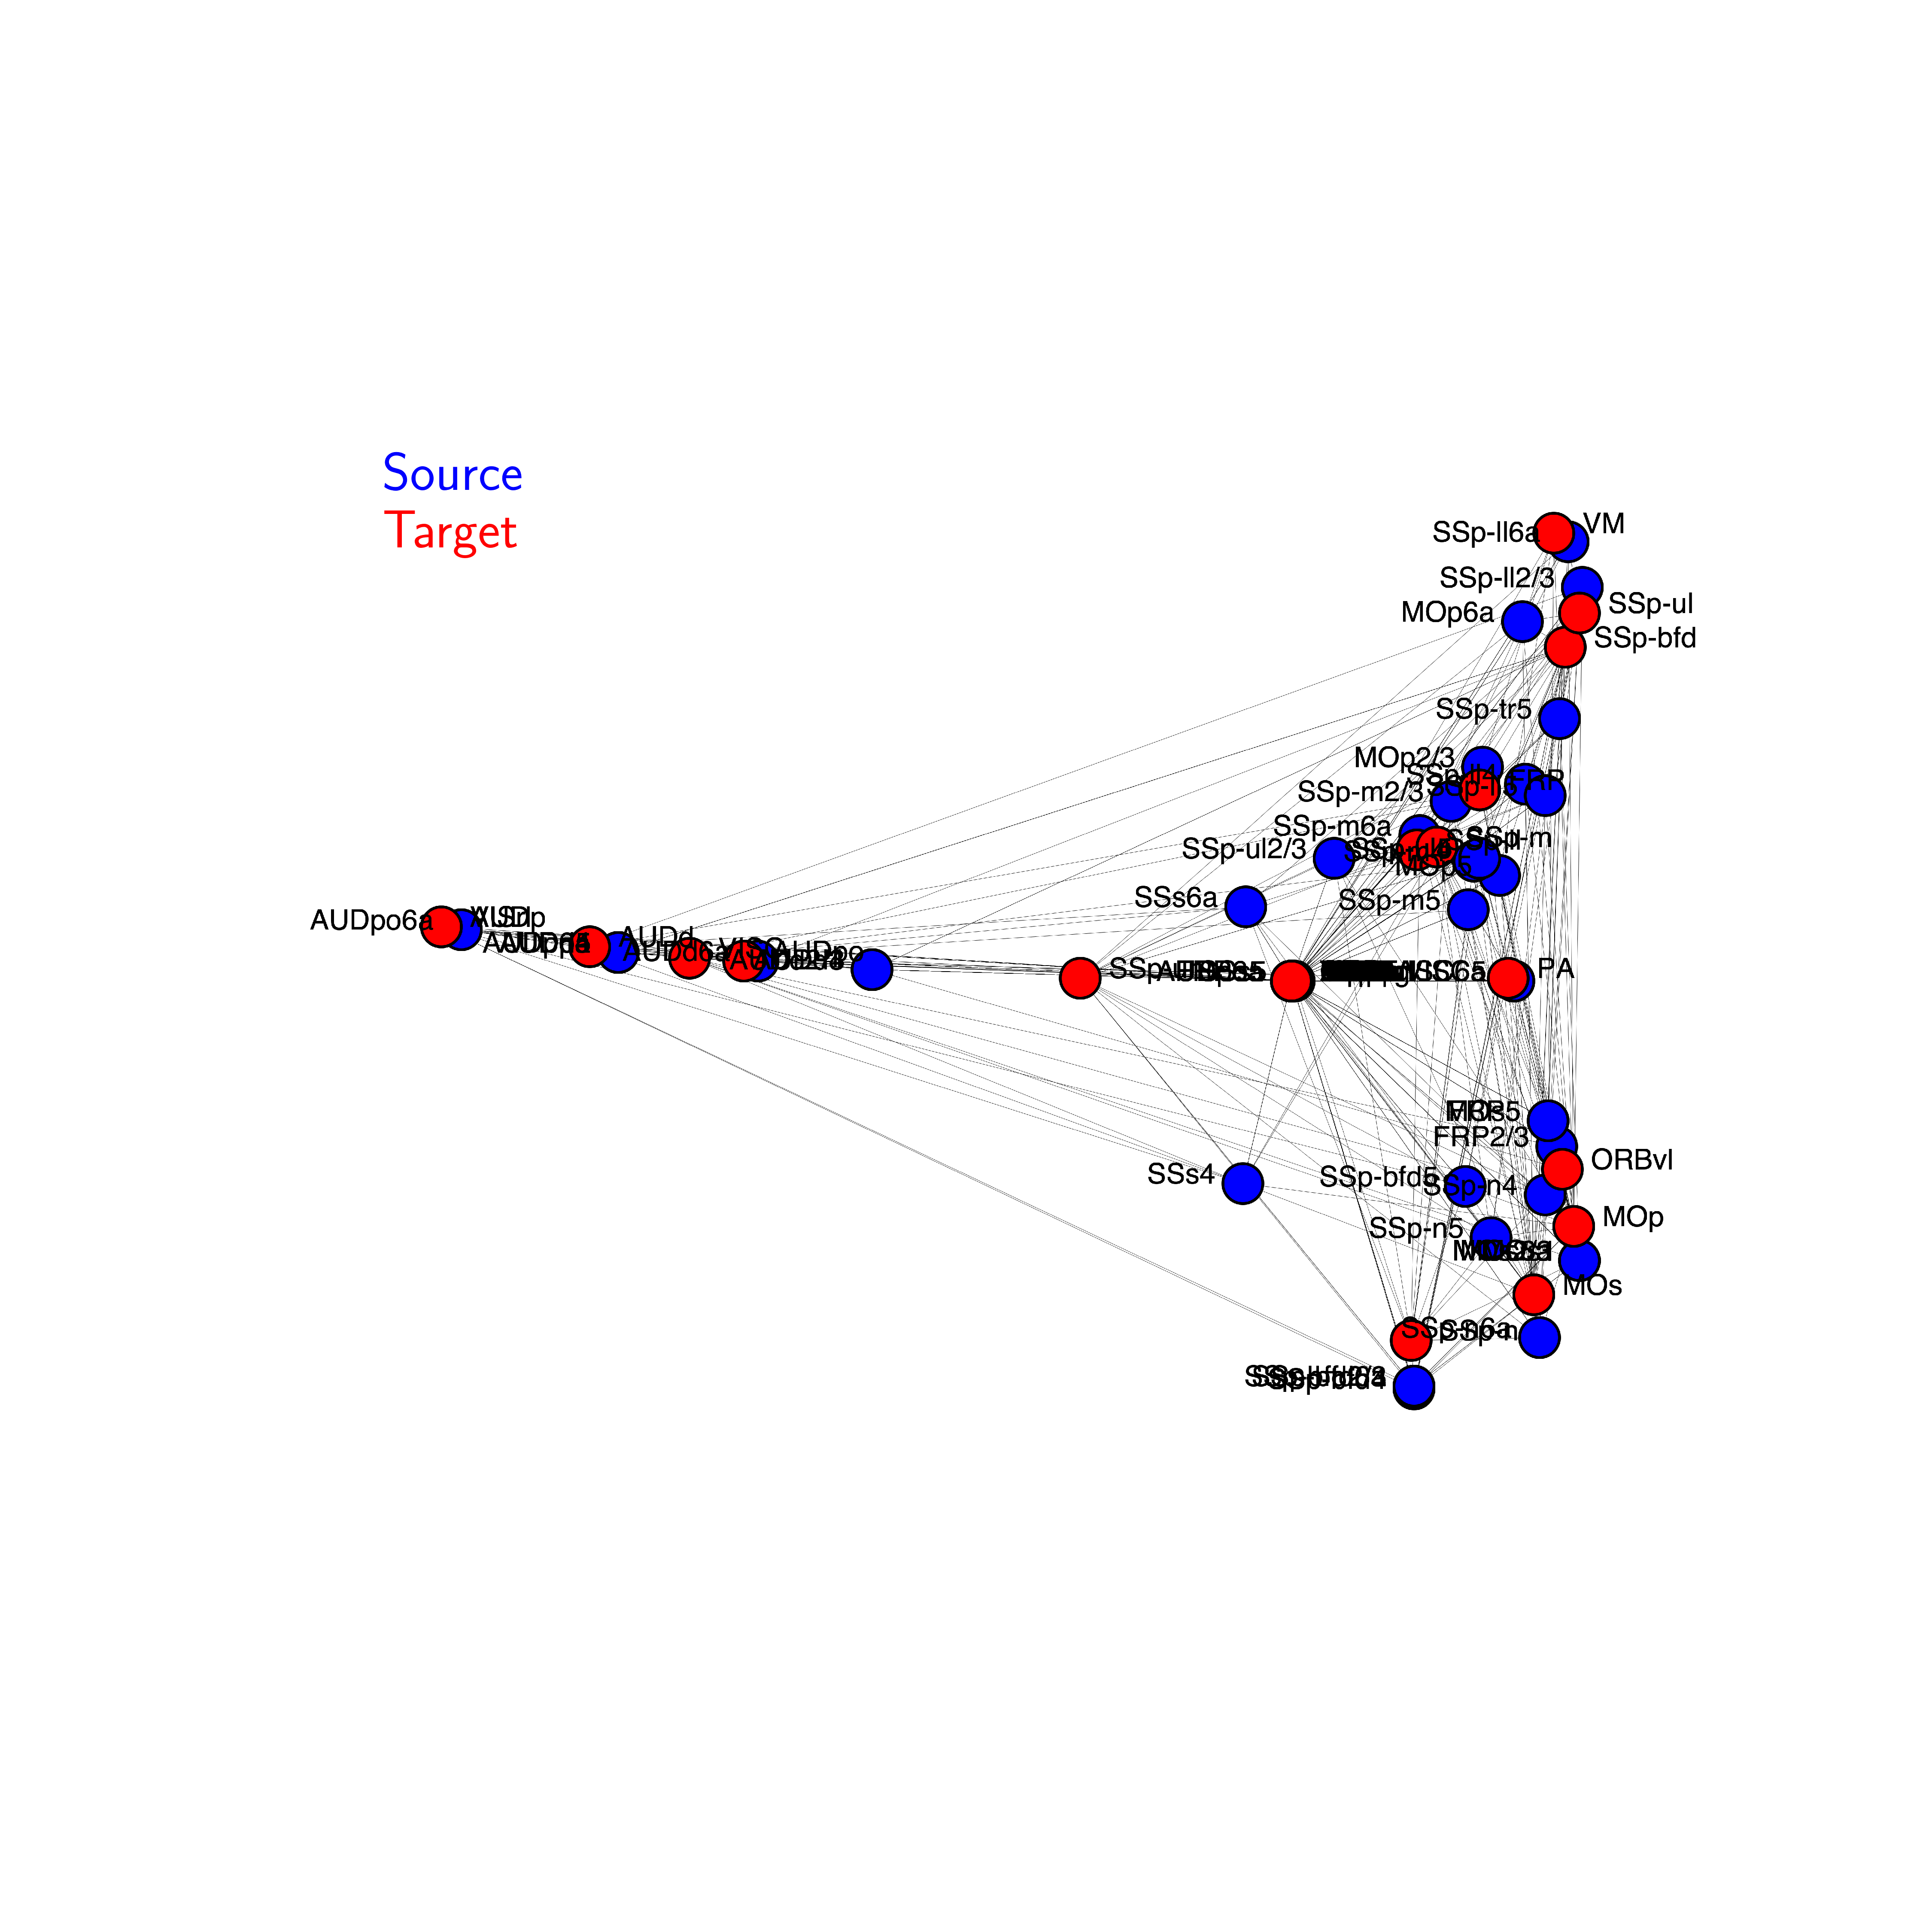
\includegraphics[width = 3in]{figs/st_graph}
    }
    } \\
     \vspace{-4cm}
    \subfloat[]{
    \adjustbox{valign=c}{
    \tiny
    \begin{tabular}{lrllll}
       
\toprule
{} &  \# Ipsilateral Leaf Targets & Top Entropy & Bottom Sparsity & Bottom Entropy & Top Sparsity \\
\midrule
Isocortex &                          51 &          CP &             BAC &            BAC &         ENTl \\
OLF       &                          11 &         TMv &             III &            III &          NaN \\
HPF       &                          15 &          IG &             EPv &             PA &          NaN \\
CTXsp     &                           7 &          TT &              FC &            APr &           TT \\
STR       &                          14 &         RPA &             ISN &            PYR &           TU \\
PAL       &                           9 &          PG &           ACVII &             GR &           MG \\
TH        &                          44 &         NOD &              DN &         SSp-ll &          SCm \\
HY        &                          44 &         CLA &              SH &            LSc &           DG \\
MB        &                          39 &         NDB &            SubG &            SGN &          SUB \\
P         &                          26 &          MT &            Acs5 &            SOC &          NDB \\
MY        &                          43 &          RT &             NaN &             OV &          EPd \\
CB        &                          18 &         ECT &             AOB &            MOB &           GU \\
\bottomrule
\end{tabular}
}
}
\vspace{-4cm}
    \subfloat[]{
    \adjustbox{valign=c}{
    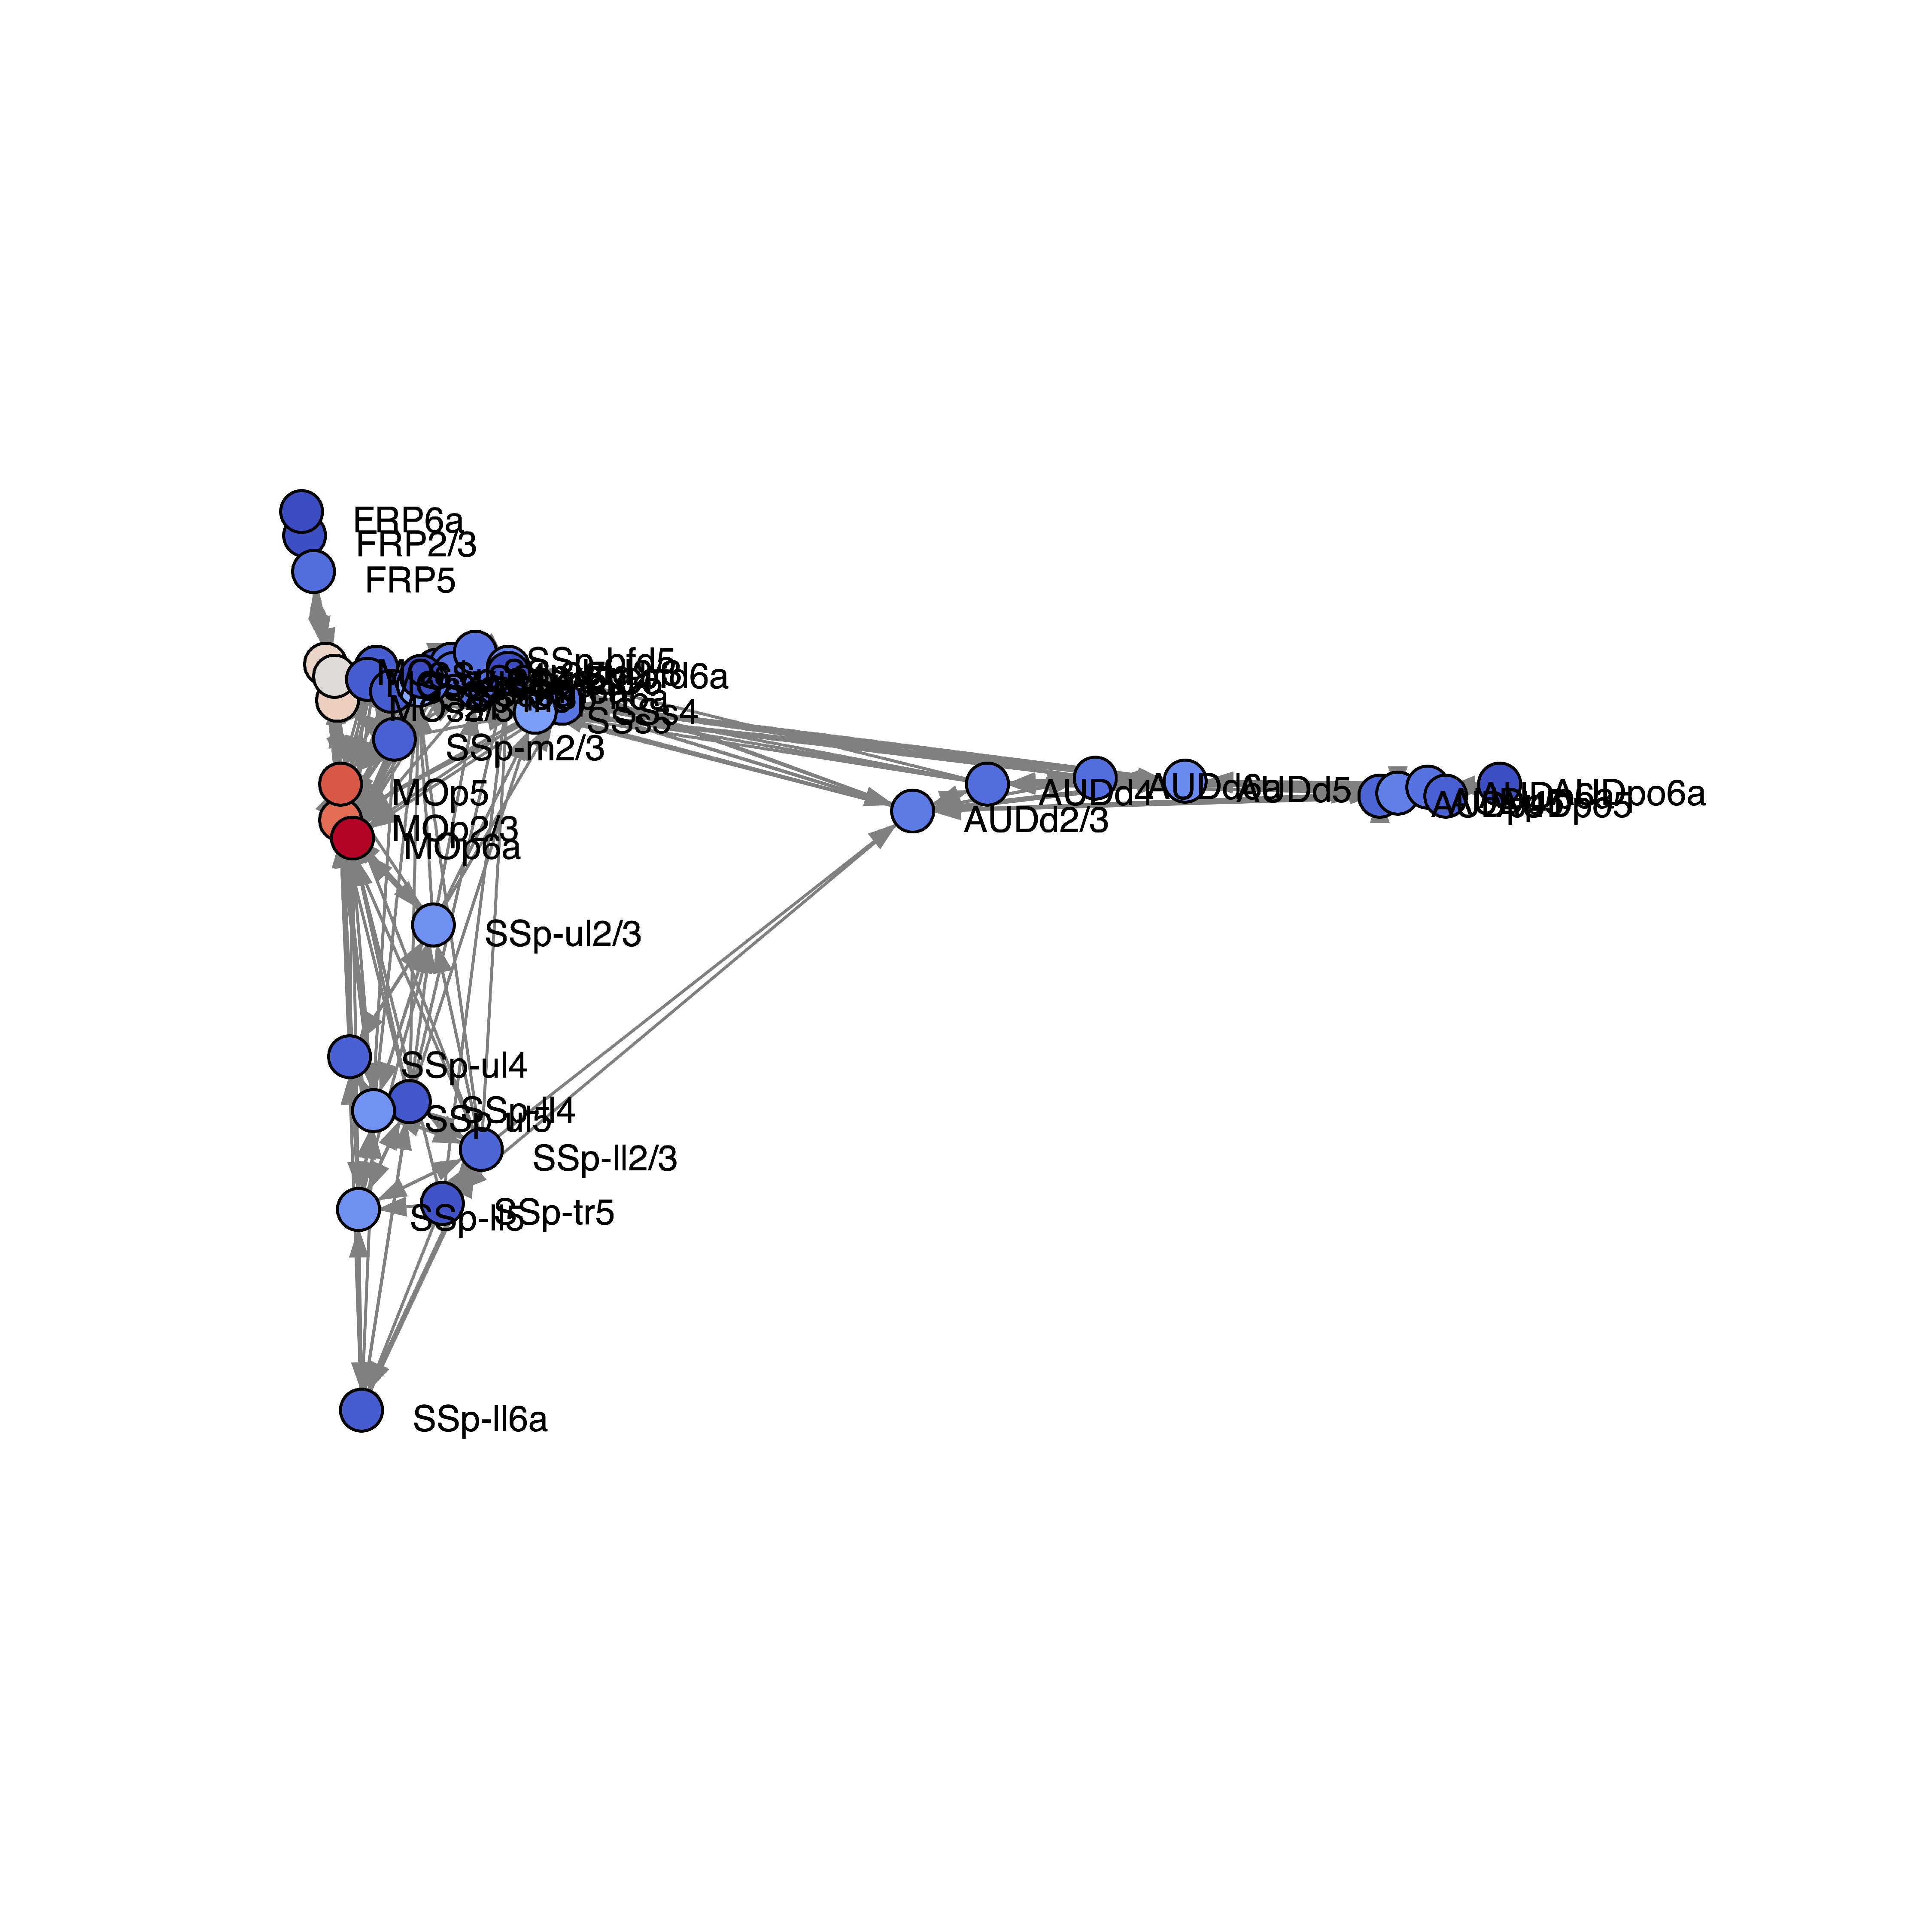
\includegraphics[width = 3in]{figs/page_graph}
    }
    }
\end{figure}



\newpage
\subsubsection{Class-specific connectivities}
The cell-type specific connectivities that we provide also conform to well-known behaviors.
Examples from the visual processing and motor control regions of the cortex are given in Figure \ref{fig:visp_mo_1201} for both wild type and several cre-lines.
Rbp4-Cre and Ntsr1-Cre target layers $5$ and $6$, respectively. As in \citet{Jeong2016-dc}, layer 5 projects to anterior basolateral amygdala (BLA) and capsular central amygdala (CEA), while layer 6 does not.

\newpage

\begin{figure}[H]
\subfloat[]{
    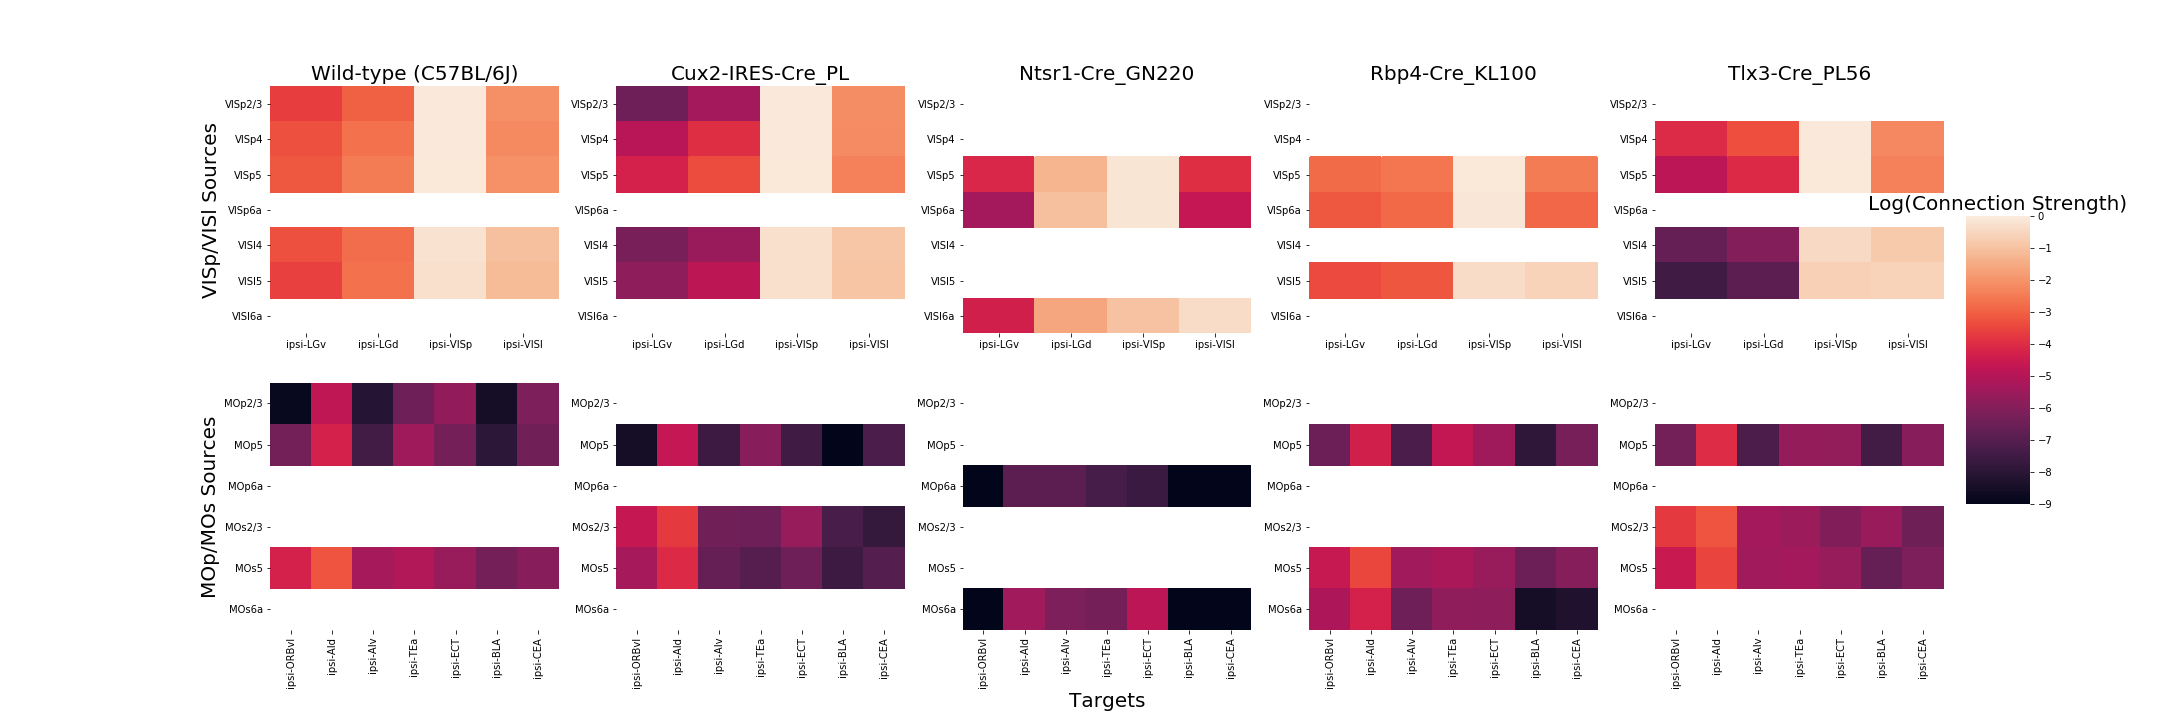
\includegraphics[width=1.\textwidth]{figs/visp_mo_1201.png}}
    \newline
 \subfloat[]{
    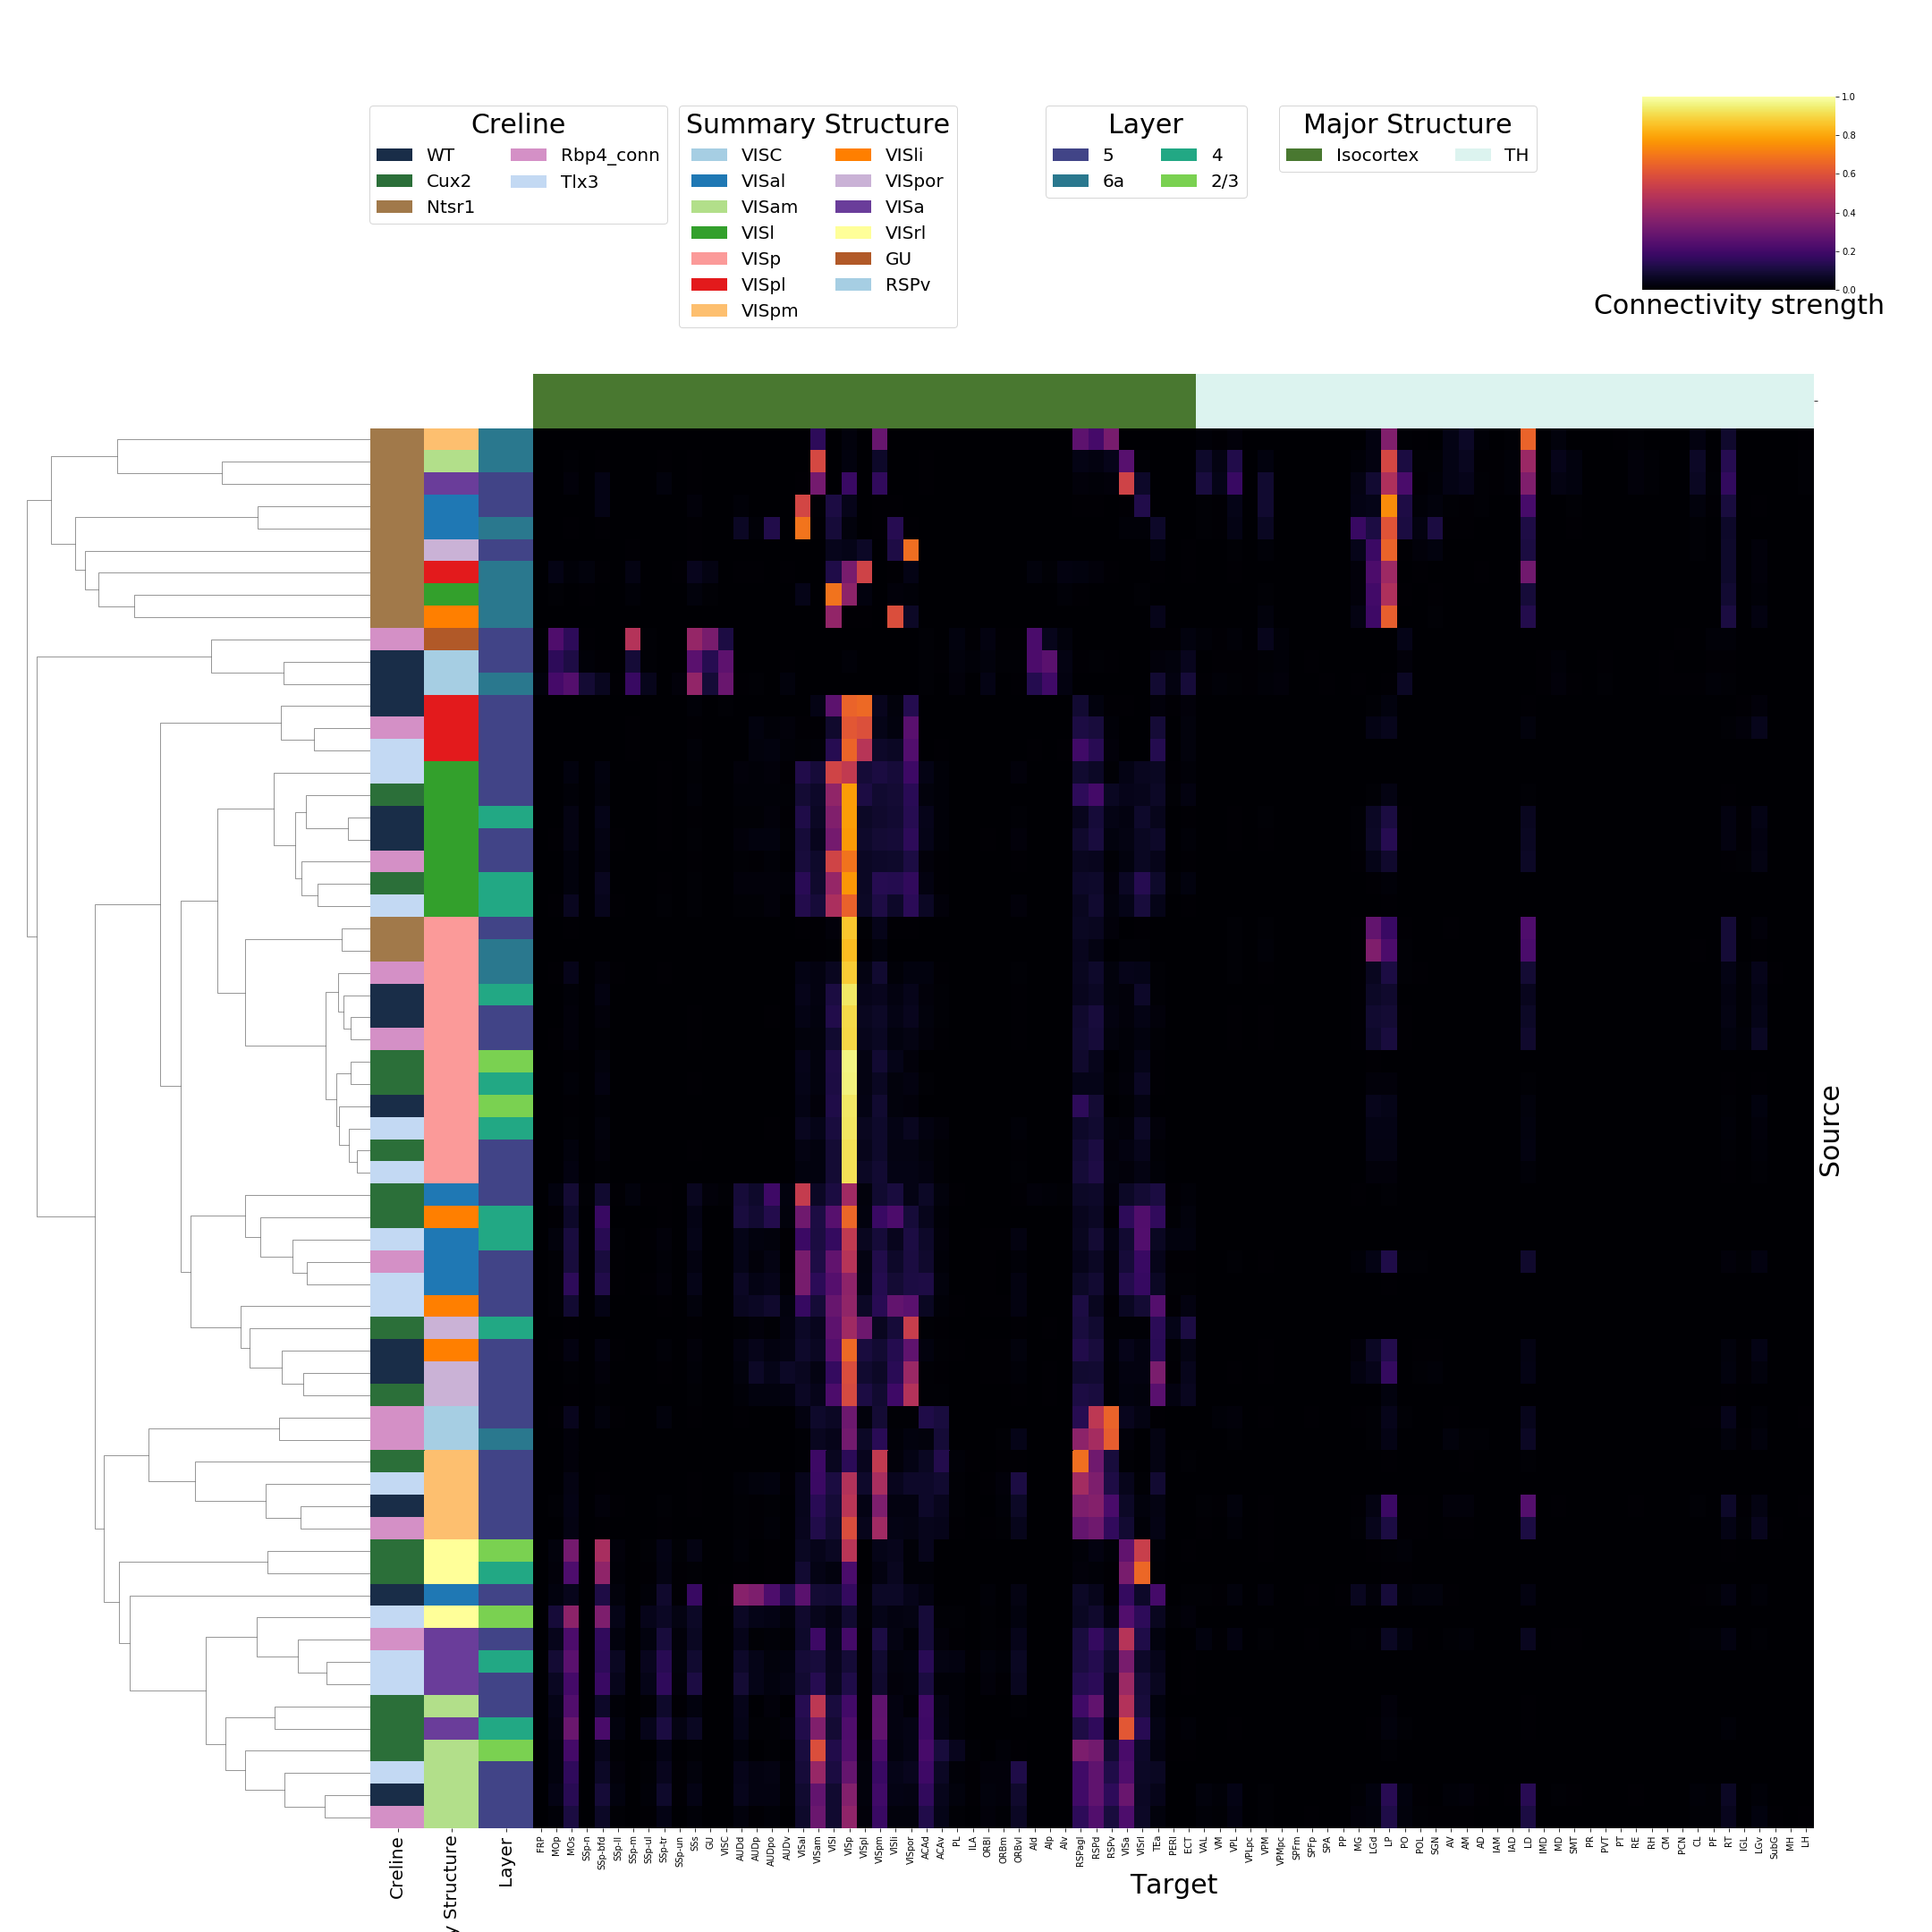
\includegraphics[width=1.\textwidth]{figs/Figure4.png}}
    \caption{   Cre-specific connection strengths from motor-cortex and visual cortex. Sources without a injection of that cre-type are blank. \skcomment{Remove 'ipsi' from columns'}}
    \label{fig:data}
\end{figure}
\newpage


\subsection{Connectivity Analyses}

%weight entropy versus accuracy

The connectivity matrix represents a collection of relatively few biological processes.
For example, certain cell-types and layers have a characteristic connectivity pattern, and structures tend to connect most strongly to the most proximal areas.
We elucidate these patterns through two types of analyses. 
First, we demonstrate cell-type specific connectivity patterns by heirarchical clustering of connectivities from multiple cre-lines, and showing that cre-line is a key factor driving the observed behavior. 
Then, we perform a different unsupervised analysis - non-negative matrix factorization - of distal wild-type connectivities, to estimate underlying overall connectivity patterns.

Figure \ref{fig:heirarchical} shows a collection of connectivity strengths generated using cre-specific models for wild-type, Cux2, Ntsr1, Rbp4, and Tlx3 cre-lines from visual signal processing leafs in the cortex to cortical and thalymic nucleii.
Heirarchical clustering is applied to sort the different source/cre combinations by the similarity of their connectivities to summary-structure targets.
This analysis shows that Ntsr1 cre-lines tend to target thalymic nucleii, in particular LP and LD \citet{Jeong2016-dc}.
However, with this exception, for the other plotted cre-lines, connectivity tends to cluster by source structure.
That the tendency for structures to connect to themselves is quite strong emphasizes the special nature of the Ntsr1-Thalymic connection in this analysis.

The overall wild-type connectivity strength matrix also displays an underlying modellable structure.
As discussed in \citet{Knox2019-ot}, one of the most basic processes underlying the observed connectivity is the tendency of each source region to predominantly project to proximal regions.
The heatmap in \ref{fig:nmf}a) shows intraregion distances clearly contains an overall pattern reminscent of the connectivity matrix in \ref{fig:connectome}.
This relationship is plotted in \ref{fig:nmf} b), showing that there exists substantial variability that would be impossible to model with low-error in a univariate model, even using the diffusion model suggested in \citet{Knox2019-ot}.
These connections are biologically meaningful, but also unsurprising, and their relative strength biases learned latent coordinate representations away from long-range structures.
For this reason, we establish a $1500 \mu m$ 'distal' threshold within which to exclude connections for our analysis.
We then apply non-negative matrix factorization (NMF) to decompose the remaining censored matrix into a relatively small number of distinct projection signals, and apply an unsupervised cross-validation method to select the optimum number of signals \skcomment{Percent error... show reconstruction? log scale?}.



\begin{comment}
\resizebox{1.5in}{!}{%
\begin{tabular}{lr}
\toprule
Estimator &     Expected-loss \\
Smoothing &              Leaf \\
Target & SS \\
\midrule
CB        &             0.042 \\
CTXsp     &             0.497 \\
HPF       &             0.087 \\
HY        &             0.221 \\
Isocortex &             0.125 \\
MB        &             0.120 \\
MY        &             0.155 \\
OLF       &             0.058 \\
P         &             0.229 \\
PAL       &             0.147 \\
STR       &             0.049 \\
TH        &             0.295 \\
\bottomrule
\end{tabular}
}

\begin{tabular}{llr}
\toprule
   & Estimator &     Expected-loss \\
   & Smoothing &              Leaf \\
   & Target & Summary Structure \\
Structure & \# Eval exps &                   \\
\midrule
CB & 4   &             0.042 \\
CTXsp & 2   &             0.497 \\
HPF & 62  &             0.087 \\
HY & 41  &             0.221 \\
Isocortex & 732 &             0.125 \\
MB & 18  &             0.120 \\
MY & 7   &             0.155 \\
OLF & 17  &             0.058 \\
P & 8   &             0.229 \\
PAL & 11  &             0.147 \\
STR & 45  &             0.049 \\
TH & 29  &             0.295 \\
\bottomrule
\end{tabular}


\newpage
\begin{table}[H]
%\small
\begin{tabular}{l|rrrrrr}
\toprule
{} &  \thead{NW w/in \\ SS} &  \thead{NW w/in \\ cre-SS combo} &   \thead{NW w/in \\ leaf} &   \thead{NW w/in \\ cre-leaf combo} &   \thead{2-stage w/in \\ SS} &  \thead{2-stage w/in \\ leaf} \\
\midrule
Isocortex &    0.197949 &              0.140132 &      0.184242 &                0.150736 &         0.123061 &           0.127477 \\
OLF       &    0.063727 &              0.074488 &      0.063727 &                0.074488 &         0.048604 &           0.055660 \\
HPF       &    0.123701 &              0.093232 &      0.112693 &                0.101307 &         0.079024 &           0.083872 \\
CTXsp     &    0.496673 &              0.496673 &      0.496673 &                0.496673 &         0.496673 &           0.496673 \\
STR       &    0.081748 &              0.063708 &      0.081748 &                0.063708 &         0.049181 &           0.048064 \\
PAL       &    0.256060 &              0.194300 &      0.256060 &                0.194300 &         0.119387 &           0.137670 \\
TH        &    0.314873 &              0.572374 &      0.314612 &                0.572254 &         0.283193 &           0.326897 \\
HY        &    0.240828 &              0.259324 &      0.240828 &                0.259324 &         0.203881 &           0.219835 \\
MB        &    0.139129 &              0.119975 &      0.129236 &                0.119420 &         0.108631 &           0.112262 \\
P         &    0.264159 &              0.238584 &      0.264159 &                0.238584 &         0.206783 &           0.228114 \\
MY        &    0.201169 &              0.224394 &      0.201169 &                0.224394 &         0.118224 &           0.163585 \\
CB        &    0.039459 &              0.049516 &      0.039459 &                0.049516 &         0.024929 &           0.038626 \\
\bottomrule
\end{tabular}
\caption{Leave-one-out cross-validation results for experiments at the summary-structure level.}
\end{table}

\newpage

\begin{table}[H]
%\small
\begin{tabular}{l|rrrrrr}
\toprule
{} &  \thead{NW w/in \\ SS} &  \thead{NW w/in \\ cre-SS combo} &   \thead{NW w/in \\ leaf} &   \thead{NW w/in \\ cre-leaf combo} &   \thead{2-stage w/in \\ SS} &  \thead{2-stage w/in \\ leaf} \\
\midrule
Isocortex &    0.308850 &              0.170937 &      0.276799 &                0.183782 &         0.157795 &           0.156463 \\
OLF       &    0.055691 &              0.065967 &      0.055691 &                0.065967 &         0.050010 &           0.045780 \\
HPF       &    0.145990 &              0.100792 &      0.127685 &                0.107282 &         0.092406 &           0.087957 \\
CTXsp     &    0.601404 &              0.601404 &      0.601404 &                0.601404 &         0.601404 &           0.601404 \\
STR       &    0.080912 &              0.060845 &      0.080912 &                0.060845 &         0.045861 &           0.046731 \\
PAL       &    0.239272 &              0.201293 &      0.239272 &                0.201293 &         0.147122 &           0.124190 \\
TH        &    0.308351 &              0.536464 &      0.309573 &                0.537646 &         0.296443 &           0.261895 \\
HY        &    0.243442 &              0.267104 &      0.243442 &                0.267104 &         0.214046 &           0.203092 \\
MB        &    0.217693 &              0.159905 &      0.193525 &                0.158817 &         0.144303 &           0.138584 \\
P         &    0.346317 &              0.250512 &      0.346317 &                0.250512 &         0.257404 &           0.235210 \\
MY        &    0.196393 &              0.222365 &      0.196393 &                0.222365 &         0.161073 &           0.115752 \\
CB        &    0.039327 &              0.049425 &      0.039327 &                0.049425 &         0.038542 &           0.024803 \\
\bottomrule
\end{tabular}
\caption{Leave-one-out cross-validation results for experiments at the leaf level.}
\end{table}
\end{comment}






%The different cre-lines display distinct connectivity patterns.


%This analysis shows that there are relatively few architypal signals underlying the overall connectome.
%Association of these patterns with the underlying biological processes is a fundamental goal in neuroscience.

%simply exhibit a collection of these patterns using several factorization methods applied to the connectivity matrix $\mathcal C$.

%Since much of the connectivity matrix can be predicted solely based off of location information.  For this reason, we subtract our the simple $\hat f_{d} c(p_1), c(p_2)$ where $\hat f$ is the estimated relation of distance between regional centroids and connectivity strength.

%, which we elucidate through n. First, projection signals cluster by target and by source; we can identify similarly behaving structures and neural targets that tend to co-occur.  Second, the specific cell-types targeted by the various cre-lines themselves generate a reduced-dimension space. Under the assumption that cell-type determines projection pattern, we can investigate which cell-types are present in which of the projecting structures.

%The choice of matrix factorization method reflects particular scientific subquestions and probabilistic interpretations. 

\newpage
 \begin{comment}
%\comment{
\begin{figure}[h]
    \centering
    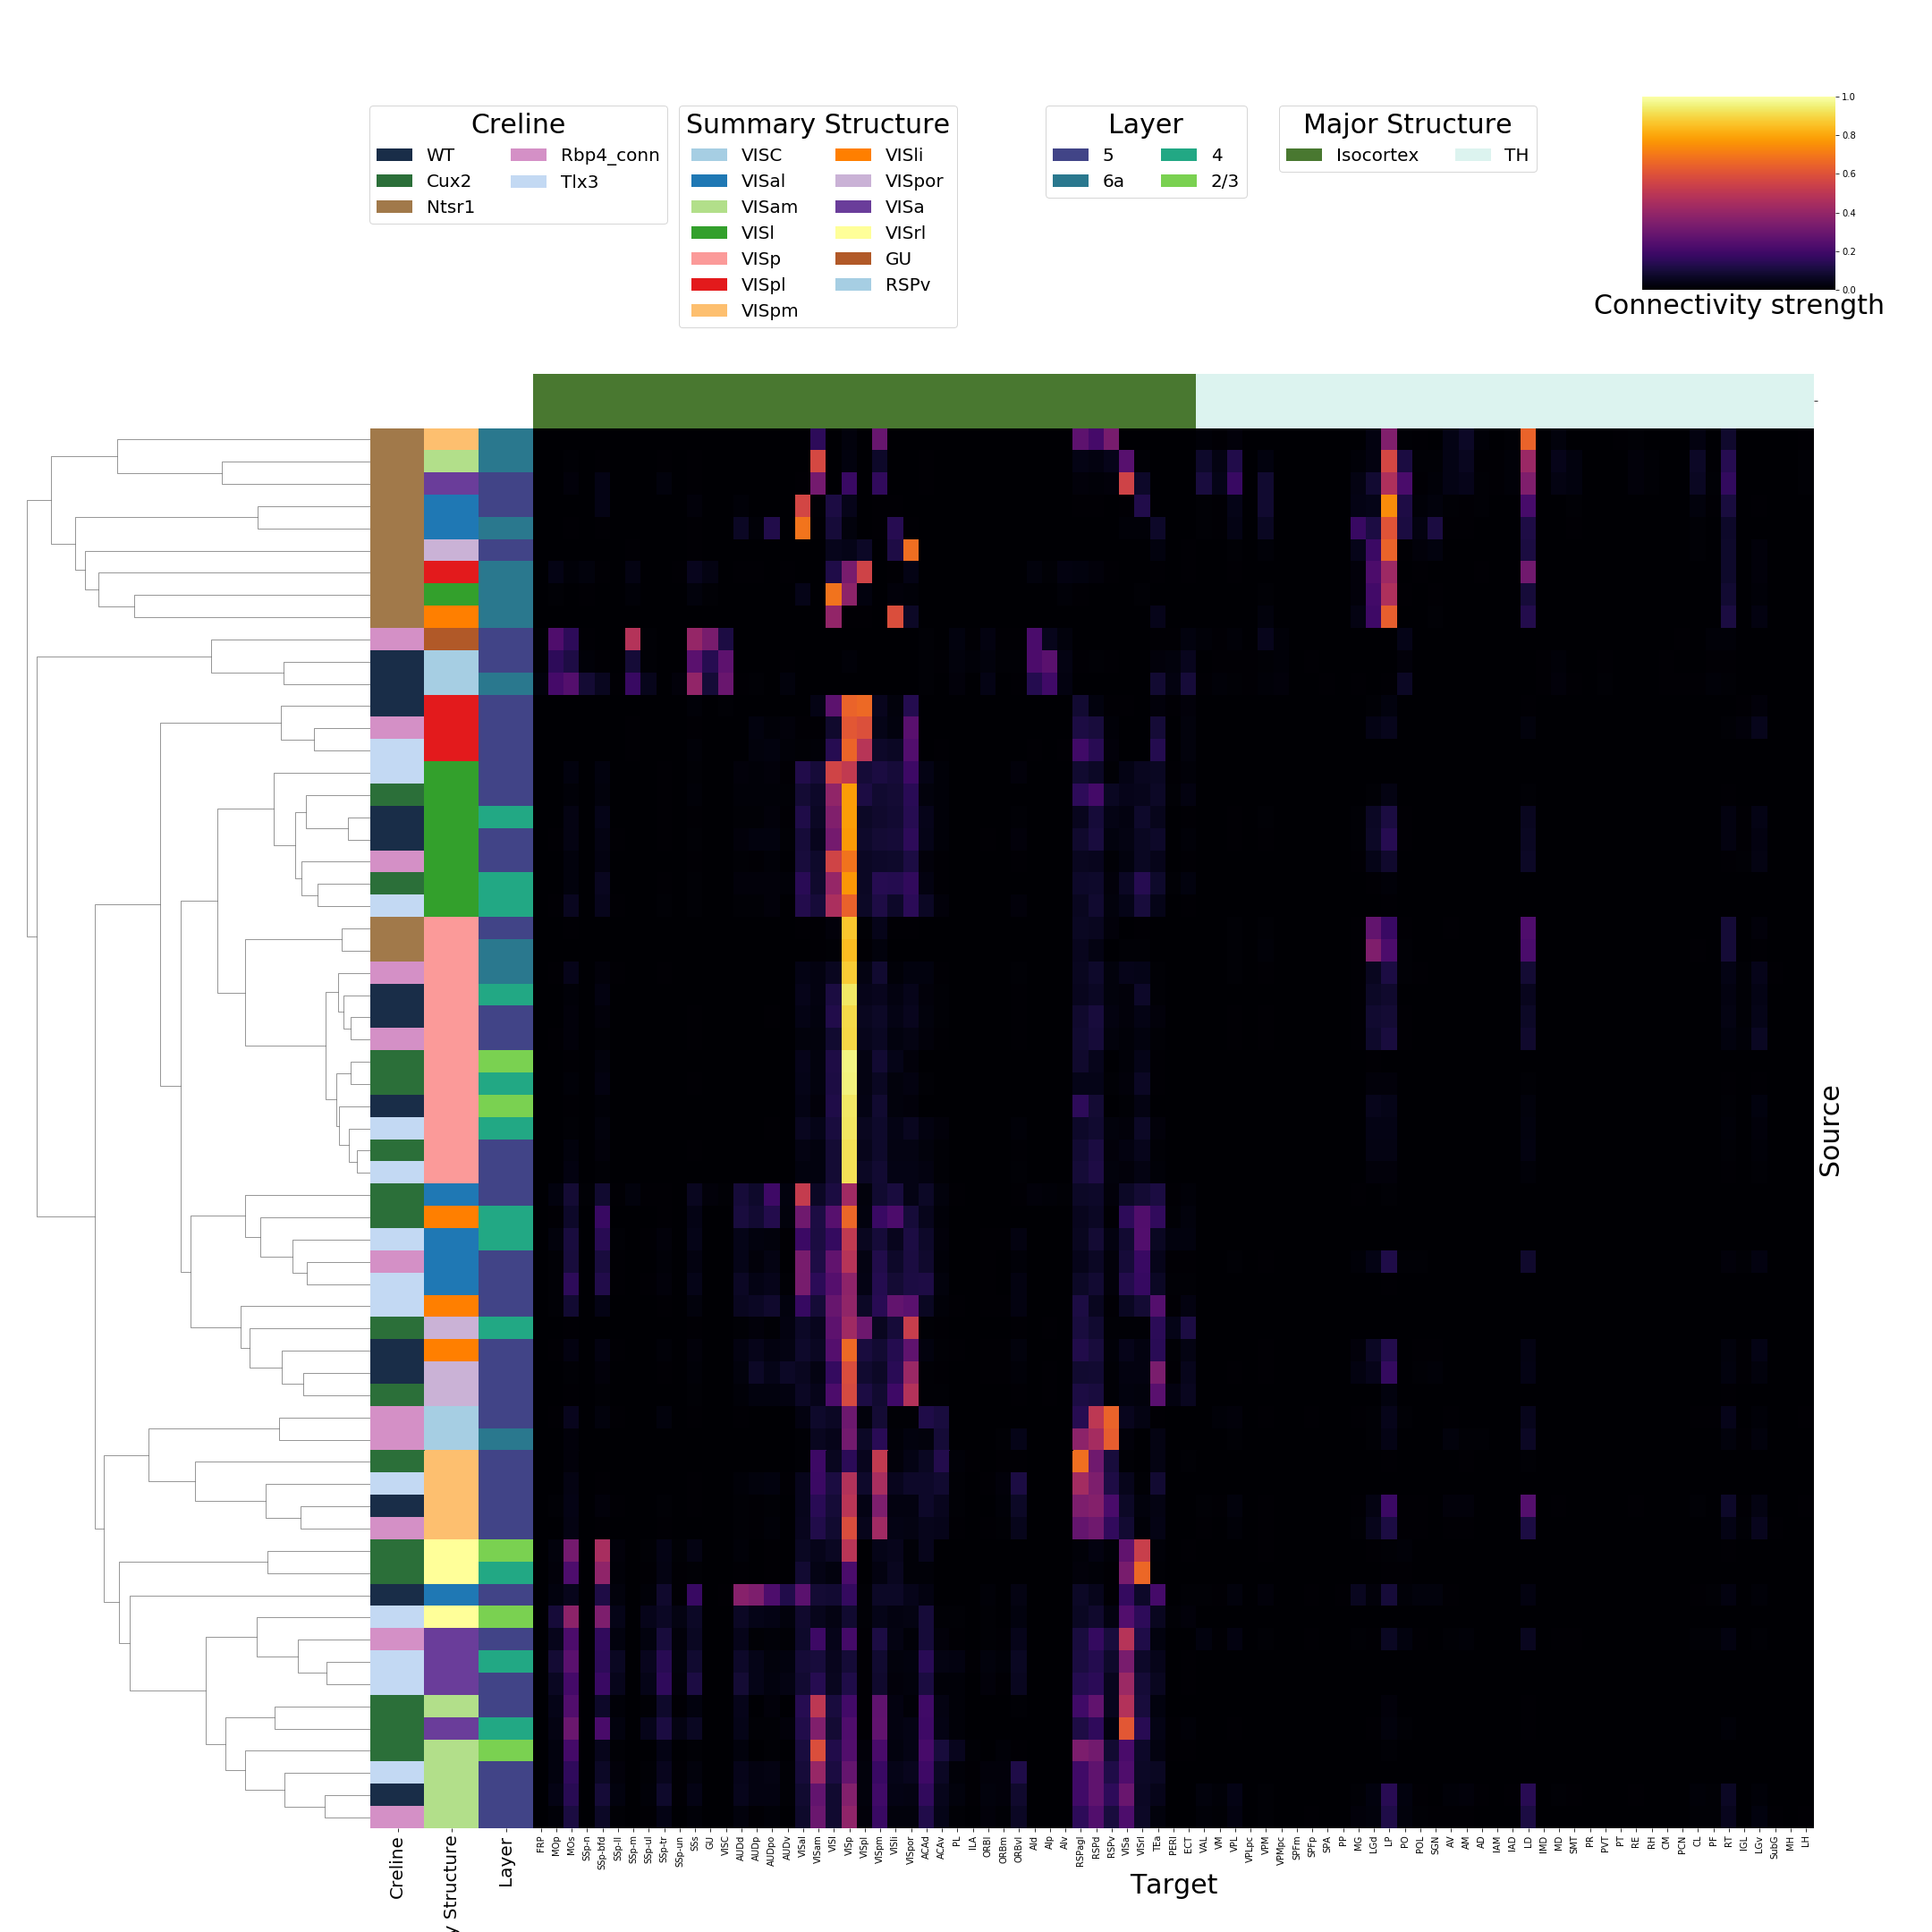
\includegraphics[width = 6in]{figs/Figure4.png}
    \caption{Heirarchical clustering of connectivity strengths from visual signal processing cell-types to cortical and thalymic targets. Cre-line, summary structure, and layer are labelled on the sources. Note that sources/cre combinations are only included if there is at least one experiment of that cre-line in that particular leaf.}
    \label{fig:heirarchical}
\end{figure}
\newpage


\begin{figure}[h]
\begin{tabular}[t]{ccc}
\subfloat[]{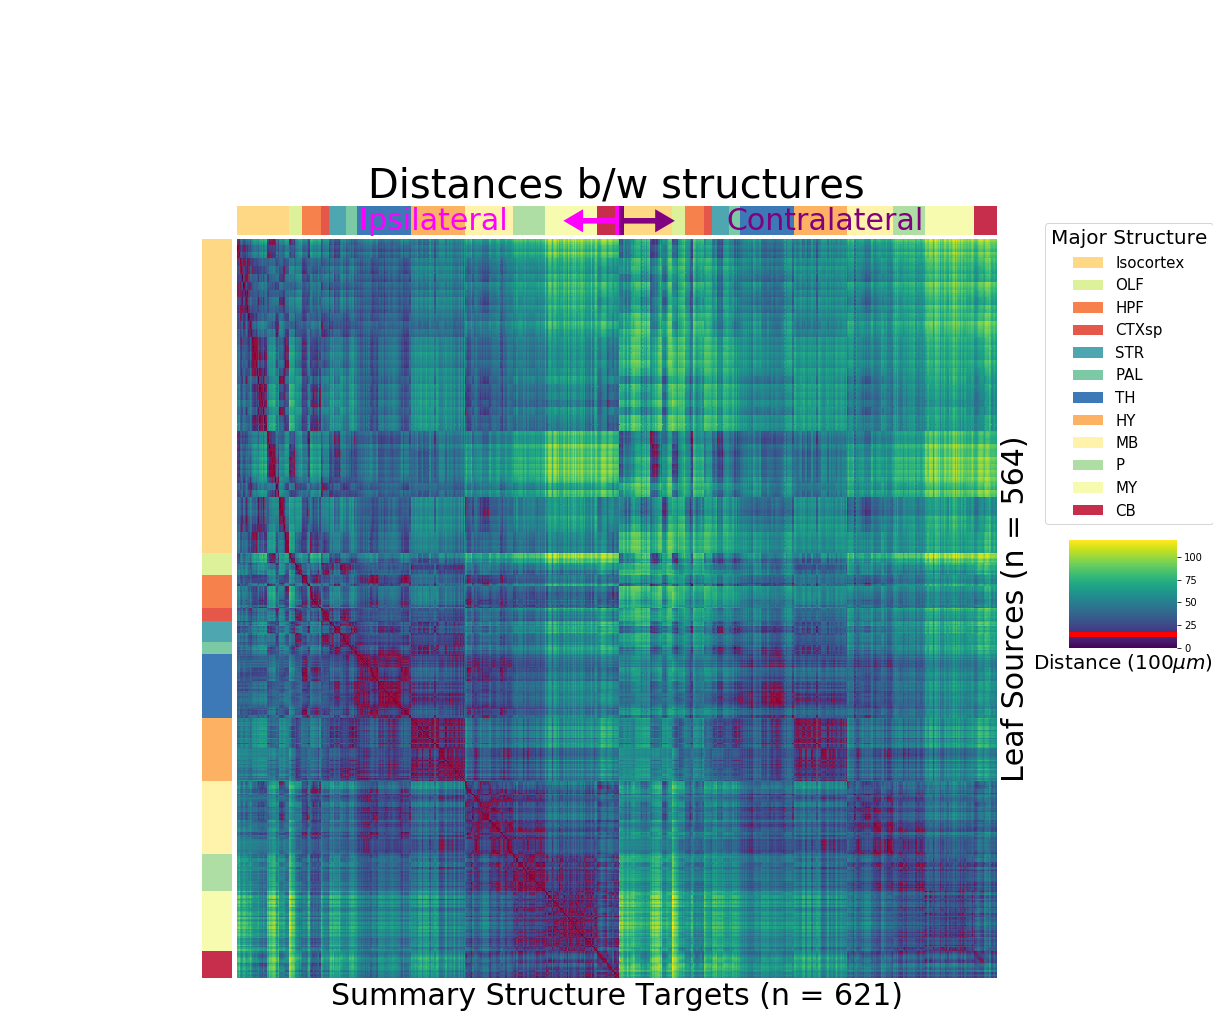
\includegraphics[width = 2in]{figs/distances_nice.png}}
& 
\vspace{1cm}
\subfloat[]{\includegraphics[width = 1.5in]{figs/figsforpres/test_train.png}} &
\subfloat[]{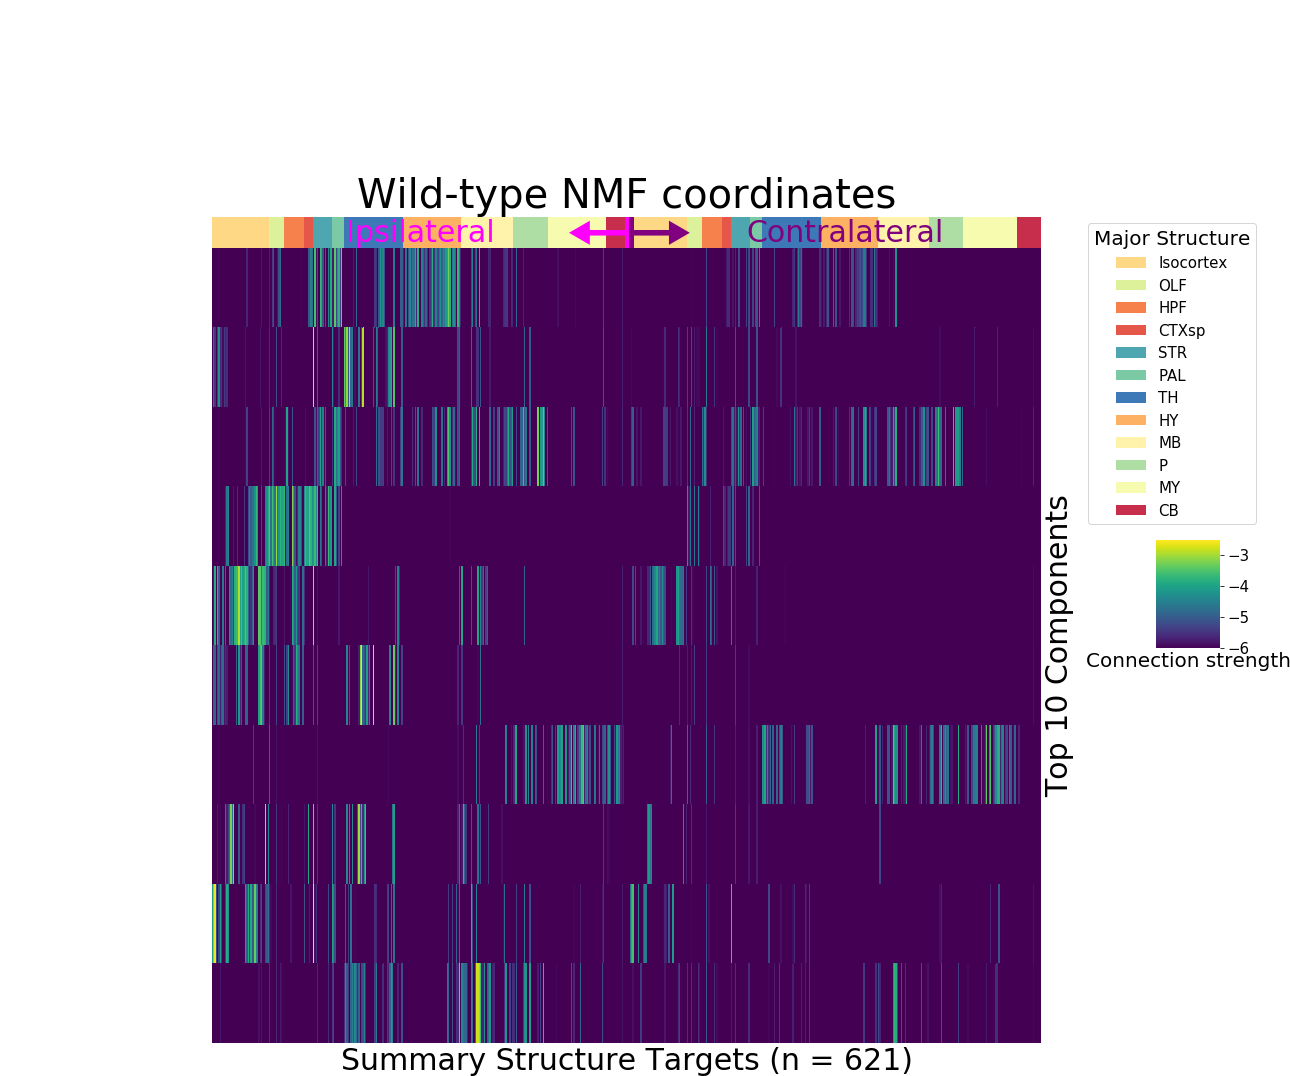
\includegraphics[width = 2in]{figs/wt_nmf_alpha0.png}}
\end{tabular}
\end{figure}

\begin{figure}[h]
    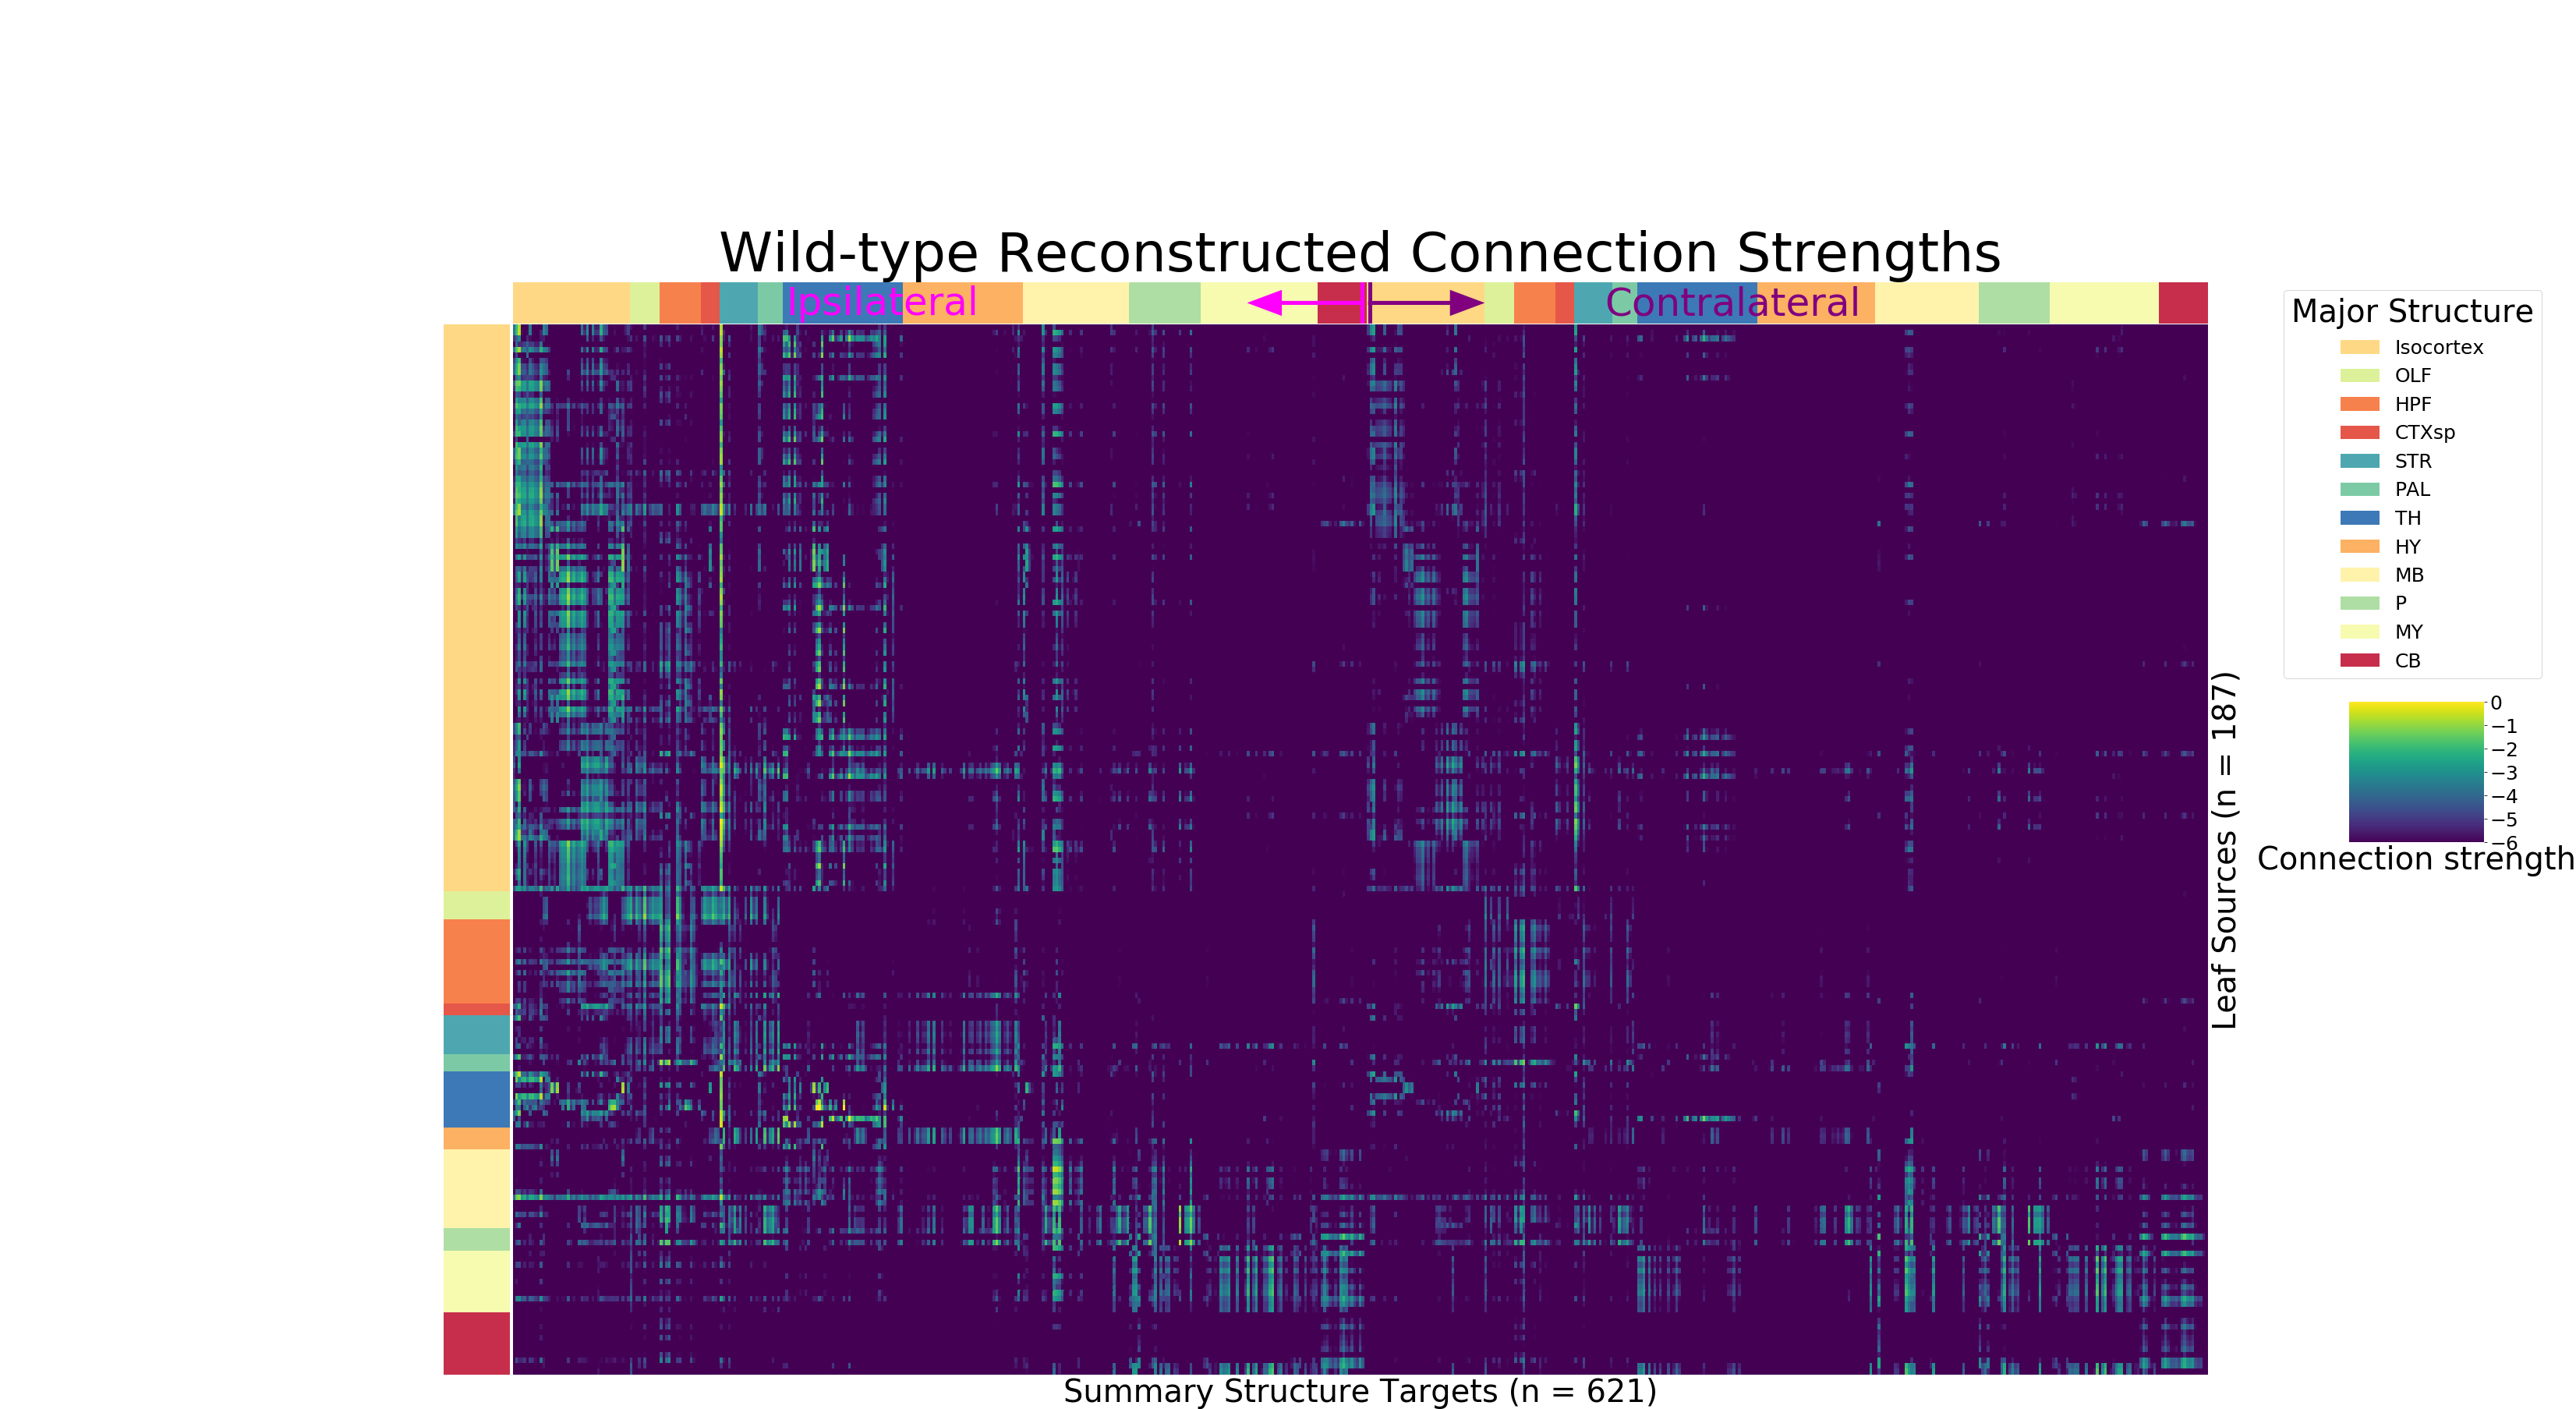
\includegraphics[width = 5in]{figs/wt_recon.png}
    %\caption{Caption}
    \label{fig:my_label}
\end{figure}
\end{comment}
%}
% \begin{figure}[h]
%     \centering
%     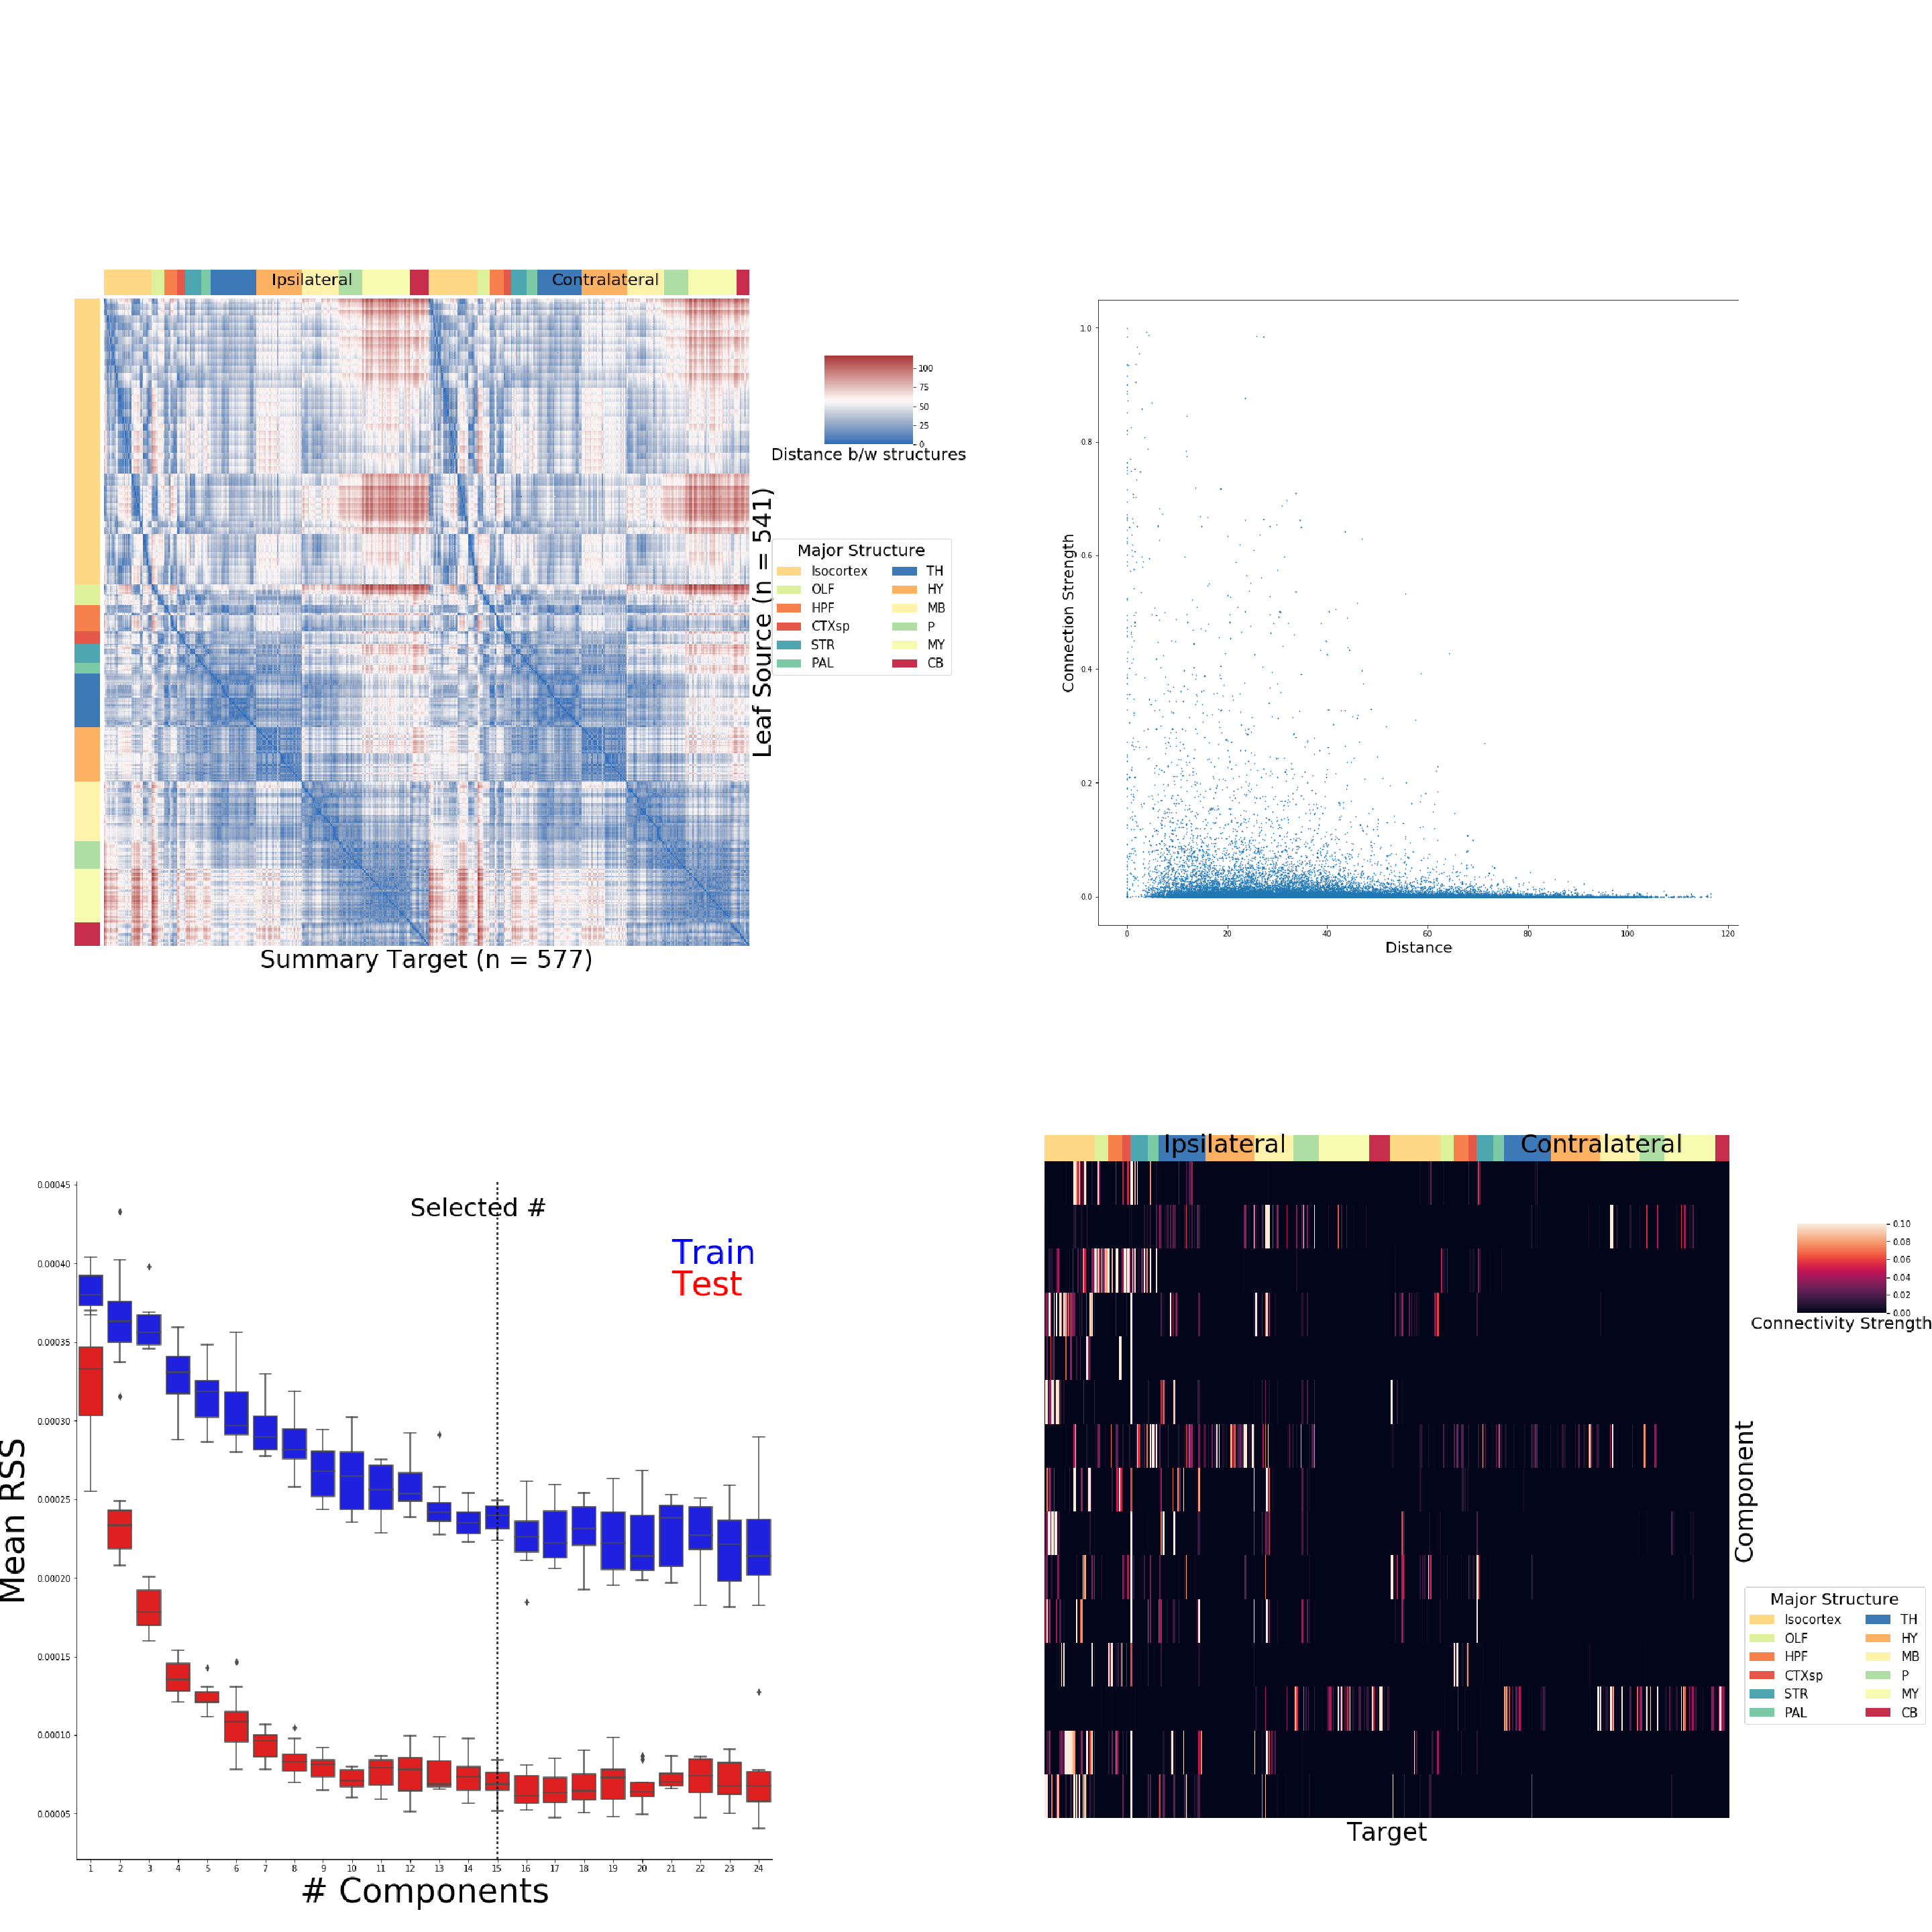
\includegraphics[width = 6in]{figs/Figure5.png}
%     \caption{a) Distances between structures \skcomment{Add units to distance legend}. b) Relation between connectivity strength and distance. c) Train error and test error of non-negative matrix factorization of non-local ($> 1500 \mu m$) connectivities. d) The top $15$ factorization components. \skcomment{Why is compressability so high}}
%     \label{fig:nmf}
% \end{figure}
% \newpage





%Our core model evaluation method is leave-one-out cross validation. This method is robust to the trivial overfitting in Nadaraya-Watson bandwidth selection. We show that incorporation of cre lines improves model performance in the following experimental set-ups. This requires at least two experiments in every experimental division, even in the 2-stage model, since leave-one-out means of each cre line may only be computed for cre-lines which are present at least twice in the leaf. This is the set up for a model trained on all data. However, for alternate models, such as the major-structure divided model from \citet{Knox2019-ot}, the potential evaluation set is larger. In order to compare between methods, we therefore restrict to the smallest set of evaluation indices, which is to say, virus-leaf combinations that are present at least twice.  This means that in some cases, our training set exceeds our evaluation set in size. 


%\begin{tabular}{lrrrr}
%{} &  Jackknife 2-stage &  Leaf average &  Creleaf average &  Creleaf NW \\
%Isocortex &           0.247344 &      0.495706 &         0.336688 &    0.300725 \\
%OLF       &           0.355304 &      0.415619 &         0.511035 &    0.550080 \\
%HPF       &           0.175599 &      0.288700 &         0.244325 &    0.252792 \\
%CTXsp     &           0.444341 &      0.444341 &         0.444341 &    0.444341 \\
%STR       &           0.339494 &      0.876627 &         0.386912 &    0.407204 \\
%PAL       &           0.221939 &      0.414942 &         0.299539 &    0.301274 \\
%TH        &           0.333870 &      0.403145 &         0.644163 &    0.644865 \\
%HY        &           0.219867 &      0.260841 &         0.303319 &    0.294789 \\
%MB        &           0.254503 &      0.431675 &         0.310175 &    0.264034 \\
%P         &           0.183399 &      0.296101 &         0.240284 &    0.240284 \\
%MY        &           0.133392 &      0.260755 &         0.316030 &    0.291915 \\
%CB        &           0.113383 &      0.565529 &         0.148914 &    0.148914 \\
%\end{tabular}


%\begin{table}[]
%    \centering
%\begin{tabular}{l|r|r|r}
%{} &         New model & Cre-specific old model & Old model\\
%Isocortex  &  0.127336 &  0.150736 &    0.184242  \\
%OLF  &  0.058567 &  0.079846 & 0.077752 \\
%HPF  &  0.079664 &  0.108270 & 0.128780\\
%CTXsp  &  0.496673 &  0.496673 & 0.496673 \\
%STR  &  0.051538 &  0.067820 & 0.081748\\
%PAL  &  0.135417 &  0.195684 & 0.256060 \\
%TH  &  0.319509 &  0.573850 &  0.314612\\
%HY  &  0.209917 &  0.259324 &  0.233678\\
%MB  &  0.112262 &  0.119420 &  0.121561 \\
%P  &  0.226793 &  0.238584 &  0.257031\\
%%MY &  0.158823 &  0.238236  &  0.193499 \\
%CB &  0.040000 &  0.049516 & 0.064922 \\
%\end{tabular} 
%\caption{Caption}
%    \label{tab:my_label}
%\end{table}


%\begin{tabular}{lr}
%{} &    Old model  \\
%0  &  0.184242 \\
%1  &  0.077752 \\
%2  &  0.128780 \\
%3  &  0.496673 \\
%4  &  0.081748 \\
%5  &  0.256060 \\
%6  &  0.314612 \\
%7  &  0.233678 \\
%8  &  0.121561 \\
%9  &  0.257031 \\
%10 &  0.193499 \\
%11 &  0.064922 \\
%\end{tabular}



% \begin{figure}[H]
%     \centering
%     \includegraphics[width = 10cm]{Figures/Connectivities/wildtype.png}
%     \caption{Caption}
%     \label{fig:wt_visp_conn}
%     %this is the old figure... update
% \end{figure}

%\begin{figure}[p]
%    \centering
%    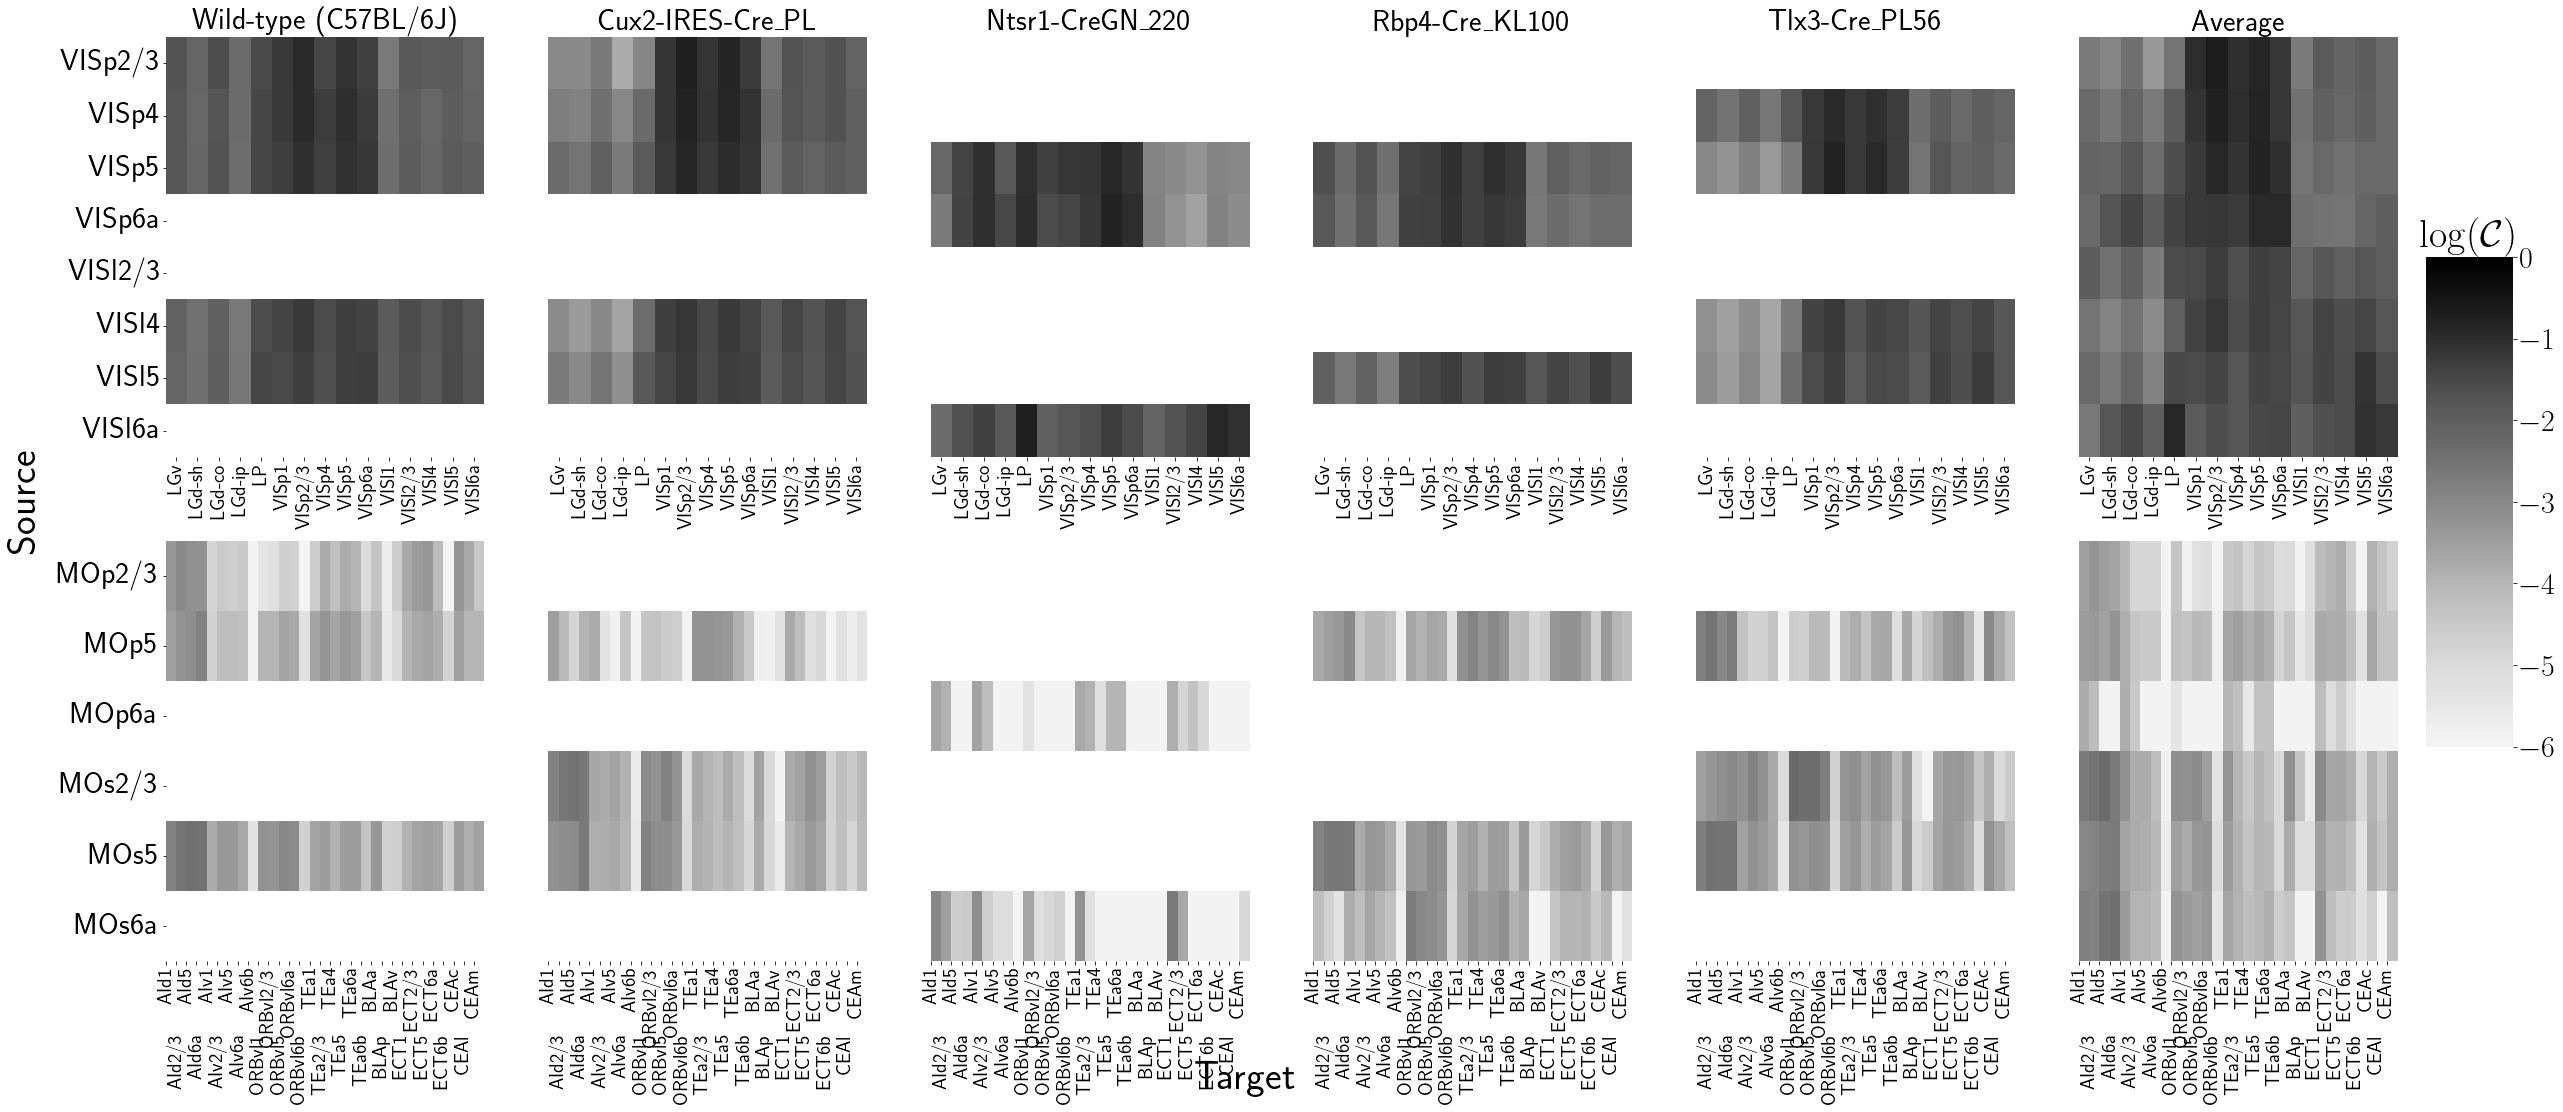
\includegraphics[width = 18cm]{figs/visp_mo.png}
%    \caption{Cre-line specific connectivity matrices for a selection of sources and targets are displayed as heatmaps. Sources without a injection of that cre-type are blank.}
%    \label{fig:my_label}
%\end{figure}


